\documentclass[a4paper]{article}
\usepackage[german,english]{babel}
\usepackage{amsmath}
\usepackage{amssymb}
\usepackage{amsthm}
\usepackage{graphicx}
\usepackage{caption}
\usepackage{centernot}
\usepackage{fontspec}
\usepackage{mdframed}
\usepackage{pxfonts}
\usepackage{wasysym}
\usepackage{framed}
\usepackage{xcolor}
\usepackage{makeidx}
\usepackage{csquotes}
\usepackage[pdfborder={0 0 0}]{hyperref}
\usepackage{stmaryrd}
\usepackage{unicode-math}
\usepackage{titlesec}
\titleformat{\paragraph}{\normalfont\itshape}{}{}{}

% okay-ish main typefaces: Alegreya, Junicode, CMU Concrete, Linux Libertine O, Libertinus Serif, URW Palladio L, Bookerly, Andada
\setmainfont{Alegreya}  % TODO \setminus is broken, \textbackslash{} is used instead
\setmathfont{cmr10}


\newcounter{lecref}[section]
\numberwithin{lecref}{section}

\theoremstyle{break}
\newmdtheoremenv[
    linecolor=white,%
    backgroundcolor=gray!10,%
    innertopmargin=0pt]{theorem}{Theorem}[lecref]

%\newtheorem{theorem}[lecref]{Theorem}
\newtheorem*{Theorem}{Theorem}
\newtheorem{example}[lecref]{Example}
\newtheorem*{Example}{Example}
\newtheorem{definition}[lecref]{Definition}
\newtheorem*{Definition}{Definition}
\newtheorem{lemma}[lecref]{Lemma}
\newtheorem*{Lemma}{Lemma}
\newtheorem{claim}[lecref]{Claim}
\newtheorem*{Claim}{Claim}
\newtheorem{remark}[lecref]{Remark}
\newtheorem*{Remark}{Remark}
\newtheorem{algorithm}[lecref]{Algorithm}
\newtheorem*{Algorithm}{Algorithm}
\newtheorem{corollary}[lecref]{Corollary}
\newtheorem*{Corollary}{Corollary}
\newtheorem{proposition}[lecref]{Proposition}
\newtheorem*{Proposition}{Proposition}


\def\ifempty#1{\def\temp{#1} \ifx\temp\empty }

% chronological structure of lectures
\newcommand{\dateref}[1]{%
  \begin{mdframed}[backgroundcolor=gray!10,innerbottommargin=0pt,innertopmargin=0pt]
    \paragraph{\textit{$\downarrow$ This lecture took place on #1.}}%
  \end{mdframed}%
}

% useful control sequences for mathematical notation
\newcommand{\Abs}[1]{\left|#1\right|}
\newcommand{\Set}[1]{\left\{#1\right\}}
\newcommand{\SetDef}[2]{\left\{#1\,\mid\,#2\right\}}
\newcommand{\IP}[2]{\left\langle#1, #2\right\rangle}
\newcommand{\Norm}[1]{\left\|{\ifempty{#1}\cdot\else#1\fi}\right\|}
\newcommand{\Max}[1]{\max{\Set{#1}}}
\newcommand{\Min}[1]{\min{\Set{#1}}}
\newcommand{\Sup}[1]{\sup{\Set{#1}}}
\newcommand{\Powerset}[1]{{\mathbb P}(#1)}
\newcommand{\IntRange}[2]{#1, \dots\ifempty{#2}\else, #2\fi}

\def\vec2#1#2{\begin{pmatrix} #1 \\ #2 \end{pmatrix}}
\def\vec3#1#2#3{\begin{pmatrix} #1 \\ #2 \\ #3 \end{pmatrix}}
\newcommand{\noproof}[1]{A proof for Theorem~\ref{#1} is not provided.}
\newcommand{\dotted}[1]{\:\dot{#1}\:}  % dot has too little margin

% German translation
\newcommand{\dt}[1]{(dt. \enquote{\foreignlanguage{german}{#1}})}

% essential control sequences
%% \xRightarrow: \xrightarrow for \rightarrow like \xRightarrow for \Rightarrow
\makeatletter
\newcommand{\xRightarrow}[2][]{\ext@arrow 0359\Rightarrowfill@{#1}{#2}}
\makeatother

\makeatletter
\def\moverlay{\mathpalette\mov@rlay}
\def\mov@rlay#1#2{\leavevmode\vtop{%
   \baselineskip\z@skip \lineskiplimit-\maxdimen
   \ialign{\hfil$\m@th#1##$\hfil\cr#2\crcr}}}
\newcommand{\charfusion}[3][\mathord]{
    #1{\ifx#1\mathop\vphantom{#2}\fi
        \mathpalette\mov@rlay{#2\cr#3}
      }
    \ifx#1\mathop\expandafter\displaylimits\fi}
\makeatother

\newcommand{\cupdot}{\charfusion[\mathbin]{\cup}{\cdot}}
\newcommand{\bigcupdot}{\charfusion[\mathop]{\bigcup}{\cdot}}


% typesetting settings
\parindent0pt
\setlength{\parskip}{.6em}

\DeclareMathOperator{\rank}{rank}
\DeclareMathOperator{\diag}{diag}
\DeclareMathOperator{\detm}{det}
\DeclareMathOperator{\perm}{perm}
\DeclareMathOperator{\sign}{sign}
\DeclareMathOperator{\degree}{deg}
\DeclareMathOperator{\im}{image}
\DeclareMathOperator{\ke}{kernel}
\DeclareMathOperator{\prop}{probability}
\DeclareMathOperator{\Hom}{Hom}
\DeclareMathOperator{\argmax}{argmax}
\DeclareMathOperator{\argmin}{argmin}
\DeclareMathOperator{\vol}{vol}  % volume
\DeclareMathOperator*{\bigtimes}{\vartimes}

% https://tex.stackexchange.com/a/110981, CC BY-SA
\makeatletter
\providecommand*{\dotcup}{%
  \mathbin{%
    \mathpalette\@dotcup{}%
  }%
}
\newcommand*{\@dotcup}[2]{%
  \ooalign{%
    $\m@th#1\cup$\cr
    \hidewidth$\m@th#1\cdot$\hidewidth
  }%
}
\makeatother

% metadata
\title{
  Measure and integration theory \\
  \large{Lecture notes, University (of Technology) Graz} \\
  based on the lecture by Wolfgang W\"oss
}
\date{\today}
\author{Lukas Prokop}

% generate index database
\makeindex


\begin{document}
\newcommand\gen{{\mathcal E}}
\renewcommand\setminus{\,{\textbackslash{}}\,} % TODO interesting: if we put this before begin{document}, it won't take effect

\maketitle
\tableofcontents

\section{Course}

\begin{enumerate}
  \item Thursday, 16:15--18:00
  \item Monday, 12:15--14:00
  \item Exam: oral, date negotiation per email, 3 examinees at once
  \item In this document, $\subset$ denotes $\subseteq$ or $\subsetneq$
  \item Literature: \enquote{Measure Theory} by Paul R. Halmos
\end{enumerate}

\dateref{2018/10/01}

\section{Sigma algebras and measures}

A measure represents the content of a set. In $R^2$, it represents the area. In $R^3$, it represents the volume. In $R^d$, we can consider the content of a subspace as dimensionwise combination of intervals:

\[ [a_1, b_1] \times \dots \times [a_d, b_d] \]

To determine the \enquote{size} of this space, we can use the product of the individual interval sizes:
\[ (b_1 - a_1) \cdot \dots \cdot (b_d - a_d) \]

Consider an geometric object as in Figure~\ref{img:jordan}.
We can approximate the size of $B$ by considering inner or outer axis-parallel boundary.
The approximation using the infimum of the outer and supremum of the inner boundary defines the Jordan measure.

The indicator function of this area ($1_B$) is Riemann-integrable.

\begin{figure}[!ht]
  \begin{center}
    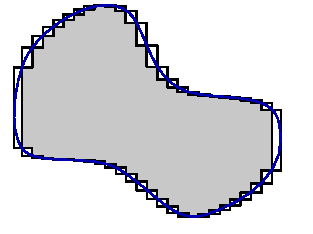
\includegraphics{img/01_jordan-measure.pdf}
    \caption{Jordan measurability of this area $B$}
    \label{img:jordan}
  \end{center}
\end{figure}

A one-point set is Jordan measurable with measure/content $0$. However, $\mathbb Q \cap [0, 1]$ is not Jordan measurable, because the indicator function is not Riemann integrable. It is desirable that the measure $\bigcupdot_{n=1}^\infty A_n = \sum_{n=1}^\infty \operatorname{measure}(A_n)$ (using pairwise disjoint union) holds true.

Modern measure theory was established by Lebesgue (1901):
\begin{enumerate}
  \item Union of countable sets ($\sigma$-additivity)
  \item arbitrary base set $X$ instead of $\mathbb R^d$, integration theory for $f: X \to \mathbb R$
\end{enumerate}

\subsection{Definition}

\index{Sigma-algebra}
Let $(\delta, \rho)$ be the non-empty base set.
$\mathcal A \subset P(X)$. A set system of subsets of $X$ is called \emph{sigma-algebra} ($\sigma$-algebra) if
\begin{enumerate}
  \item $X \in \mathcal A$
  \item $A \in \mathcal A \implies A^C = X \setminus A \in \mathcal A$
  \item $A_n \in \mathcal A$ ($n \in \mathbb N$) $\implies \bigcup_{n=1}^\infty A_n \in \mathcal A$
\end{enumerate}

Properties 1 and 2 implies that $\emptyset \in \mathcal A$.

\index{Measurable space}
\index{Measure}
A \emph{measurable space} is given by $(X, \mathcal A)$. A \emph{measure} $\mu: \mathcal A \to [0, \infty]$ is defined by
\begin{enumerate}
  \item $\mu(\emptyset) = 0$
  \item If $A_n \in \mathcal A$ ($n \in \mathbb N$), pairwise disjoint, then
    \[ \implies \mu\left(\bigcup_{n=1}^\infty A_n\right) = \sum_{n=1}^\infty \mu(A_n) \]
\end{enumerate}
\index{Measure space}
A \emph{measure space} is given with $(X, \mathcal A, \mu)$.

\begin{Remark}
  \begin{itemize}
    \item $\mu$ is called probability space if $\mu(X) = 1$
    \item $\mu$ is called finite measure if $\mu(X) < \infty$
    \item $\mu$ is called $\sigma$-finite if $X = \bigcup_{n=1}^\infty A_n$ with $A_n \in \mathcal A$ and $\mu(A_n) < \infty$ (e.g. real axes decomposes into intervals of length $1$)
  \end{itemize}
\end{Remark}

Examples:
\begin{enumerate}
  \item $X$ is at most countable, then mostly $\mathcal A = \Powerset{X}$.
    Then it suffices to know, $\mu(\Set{x}) \in [0, \infty)$.
    Then we denote $\mu(x) = \mu(\Set{x})$ with $x \in X$.
    \[ \mu(A) = \sum_{x \in A} \mu(x) \]
    e.g. $\mu(x) = 1 \forall x \in X$ in case of a \emph{counting measure}.
    \index{Counting measure}
  \item If $X$ is uncountable, e.g. $\mathbb R^d$, then it is not recommended to use $\Powerset{X}$. So what about $A$? Consider for example $\mathbb R^d$. All $[a_1, b_1] \times \dots \times [a_d, b_d]$ should be elements of $\mathcal A$
\end{enumerate}

\subsection{Simple properties of sigma-algebras}

\begin{enumerate}
  \item $\emptyset \in \mathcal A$
  \item $A_1, \dots, A_n \in \mathcal A \implies \bigcup_{k=1}^n A_k \in \mathcal A$
  \item $A_n \in \mathcal A$ ($n \in \mathbb N$) or $\IntRange{}{N} \implies \bigcap_{n \in \mathbb N} A_n \in \mathcal A$ (deMorgan) \\
    $\bigcap_{n} A_n = \left(\bigcup_n A_n^C\right)^C$
  \item $A, B \in \mathcal A \implies A \setminus B \in \mathcal A$, $A \triangle B = A \setminus B \lor B \setminus A$
\end{enumerate}

\index{Generating set}
\index{Generator}
\begin{definition}[Generating set]
  Let $\gen \neq \emptyset$ with $\gen \subset \Powerset{X}$ be the \emph{generator} (generating set) of the $\sigma$-algebra. $\sigma(\gen)$ is the smallest $\sigma$-algebra over $X$ which contains $\gen$.
  \[
    = \bigcap \Set{
      \tilde A: \tilde A \text{ is the } \sigma-\text{algebra over } X \text{ with } \gen \subset \tilde{\mathcal A}
    }
  \]
  This set is non-empty because $\Powerset{X}$ is the $\sigma$-algebra for all $X$ and $\gen \subset \Powerset{X}$
\end{definition}

\begin{lemma}
  If $\mathcal A_i$ with $i \in I$ is a family of $\sigma$-algebras,
  then $\bigcap_{i \in I} \mathcal A_i$ is a $\sigma$-algebra over $X$.
\end{lemma}

Immediate:
\begin{enumerate}
  \item if $\gen_1 \subset \gen_2$ ($\implies \gen_1 \subset \sigma(\gen_2)$), then $\sigma(\gen_1) \subset \sigma(\gen_2)$
  \item if additionally $\gen_2 \subset \sigma(\gen_1)$, then $\sigma(\gen_1) = \sigma(\gen_2)$
\end{enumerate}

Example:
\[ X = \bigcup_{n \in I} E_n \neq \emptyset \qquad I = \mathbb N \text{ or } \{\IntRange1N\} \]
\[ \gen = \SetDef{E_n}{n \in I} \qquad \sigma(\gen) = \SetDef{\bigcup_{n \in J} E_n}{J \subset I} \]
\begin{enumerate}
  \item Is a $\sigma$-algebra
  \item If $\gen \subset \tilde{\mathcal A}$, then $\SetDef{\bigcup_{n \in J} E_n}{J \subset I} \subset \tilde{\mathcal A}$
\end{enumerate}

\begin{Definition}
  $(X, d)$ is a metric space.
  Borel-$\sigma$-algebra $\sigma(\mathcal O)$.
  $\mathcal O$ is the set of open sets in a metric space
\end{Definition}

\begin{Example}
  Consider $\mathbb R^d$. $\mathcal B_{\mathbb R^d}$ denotes the Borel $\sigma$-algebra.
  \begin{enumerate}
    \item $\gen_1 = \Set{\text{open sets}}$
    \item $\gen_2 = \Set{\text{closed sets}}$
    \item $\gen_3 = \Set{(a_1, b_1) \times \dots \times (a_d, b_d): a_i, b_i \in \mathbb R, a_i < b_i}$ is a parallelepiped
    \item $\sigma(\gen_1) = \sigma(\gen_2) = \sigma(\gen_3) = \mathcal B_{\mathbb R^d}$
    \item $\sigma(\gen_3) = \mathcal B_{\mathbb R^d}$ because every open set is a countable union of open (or left half-open) parallelepipeds
  \end{enumerate}
\end{Example}
\[ \gen_3 \subset \gen_1 \subset \sigma(\gen_3) \]
\[ \gen_4 = \SetDef{(a_1, b_1] \times \dots \times (a_d, b_d]}{a_i, b_i \in \mathbb R, a_i < b_i} \]
\[ (a, b) = \bigcup_{n=1}^\infty (a, b - \frac1n] \]
\[ \gen_5 = \SetDef{(-\infty, b_1) \times \dots \times (-\infty, b_d]}{b_i \in \mathbb R} \text{ because } \gen_4 \subset \sigma(\gen_5) \]
If $d=1$, $(a, b] = (-\infty, b] \setminus (-\infty, a]$. Recognize that $A \setminus B = (A \cap B^C)$. \\
If $d=2$,
\[ (a_1, b_1] \times (a_2, b_2] = (-\infty, b_1] \times (-\infty, b_2] \setminus (-\infty, a_1] \times (-\infty, b_2) \setminus (-\infty, b_1] \times (-\infty, a_2] \]

\index{Trace $\sigma$-algebra}
\begin{Definition}
  $(X, \mathcal A)$ is a measurable space, $B \in \mathbb A$ is a trace $\sigma$-algebra over $B$. $\SetDef{A \in \mathcal A}{A \subset B}$
\end{Definition}

\index{Measurable maps}
\begin{Definition}
  $\varphi: (X_1, \mathcal A_1) \to (X_2, \mathcal A_2)$ is called measurable
  $\iff \varphi^{-1}(A_2) \in \mathcal A_1 \forall A_2 \in \mathcal A_2$
\end{Definition}

\begin{Remark}
  In general $\varphi$ is a map from $X_1$ to $X_2$.
  $\mathcal A_1$ and $\mathcal A_2$ are mentioned to clarify that the map depends on the chosen algebra.
\end{Remark}

\begin{Remark}
  $(X_1, d_1) \to (X_1, d_2)$ on metric spaces is continuous iff $\varphi^{-1}(O_2) \in \mathcal O_1 \forall O_2 \in \mathcal O_2$ where $\mathcal O_1, \mathcal O_2$ are sets of open sets.
\end{Remark}

\begin{Remark}
  Measurable maps are a much stronger statement than continuity, because they cover much more sets than open ones.
\end{Remark}

\begin{lemma}
  The composition of measurable maps is measurable.
  \[ \varphi: (X_1, \mathcal A_1) \to (X_2, \mathcal A_2) \text{ measurable} \]
  \[ \psi: (X_2, \mathcal A_2) \to (X_2, \mathcal A_2) \text{ measurable} \]
  \[ \implies \psi \circ \varphi: (X_1, \mathcal A_1) \to (X_3, \mathcal A_3) \text{ measurable} \]
\end{lemma}
\begin{proof}
  Show that $(\psi \circ \varphi)^{-1} (\mathcal A_3) \in \mathcal A_1$ is trivial.
\end{proof}

\begin{theorem}
  Let $\gen_2$ be a generator of $\mathcal A_2$. Then $\varphi: (X_1, \mathcal A_1) \to X_2$ is measurable in regards of $\mathcal A_2$ iff $\varphi^{-1}(E_2) \in \mathcal A_1 \forall E_2 \in \gen_2$
\end{theorem}
\begin{proof}
  \begin{description}
    \item[$\implies$] is immediate
    \item[$\impliedby$] $\tilde{\mathcal A_2} = \SetDef{A_2 \in \mathcal A_2}{\varphi^{-1}(A_2) \in \mathcal A_1}$ is a $\sigma$-algebra over $X_2$. $\gen_2$ is a TM of this $\sigma$ algebra.
    \[ \implies \mathcal A_2 = \sigma(\gen_2) \subset {\tilde{\mathcal A}}_2 \]
  \end{description}
\end{proof}

\begin{example}
  $f: \mathbb R \to \mathbb R$ is monotonically increasing
  \[ f^{-1}(-\infty,b] = \SetDef{x}{f(x) \leq b} = (-\infty, c) \in \mathcal B \]
  Thus, $f$ is measurable.
\end{example}

\begin{Remark}
  $\overline{\mathbb R} \coloneqq \mathbb R \cup \Set{-\infty, +\infty}$
\end{Remark}

\begin{example} \hfill{}
  \[ \mathcal B_{\overline{\mathbb R}} = \SetDef{B, B \cup \Set{-\infty}, B \cup \Set{+\infty}, B \cup \Set{+\infty, -\infty}}{B \in \mathcal B_{\mathbb R}} \]
  $f_1, \dots, f_n: \mathbb R \to \overline{\mathbb R}$ measurable in $(X, \mathcal A)$ and $f = \Max{f_1, \dots, f_n}$
  \[ f: \mathbb R \to \overline{\mathbb R} \qquad x \mapsto \max\Set{f_1(x), \dots, f_n(x)} \]
  \begin{align*}
    f^{-1}([-\infty, b]) &= \SetDef{x}{f(x) \leq b} \\
      &= \SetDef{x}{f_k(x) \leq b, k = 1, \dots, n} \\
      &= \bigcap_{k=1}^n \SetDef{x}{f_k(x) \leq b} \in \mathcal B
  \end{align*}
  Analogously for the minimum.
  Therefore $f$ is measurable.
\end{example}

\begin{example}
  The same applies to countably many functions.
  Let $f_n: \mathbb R \to \overline{\mathbb R}$ be measurable with $n \in \mathbb N$.
  Then $f: \sup\SetDef{f_n}{n \in \mathbb N}$ is measurable.
  \begin{align*}
    f^{-1}([-\infty, b]) &= \SetDef{x}{\sup\Set{f_n(x)} \leq b} = \SetDef{x}{f_n(x) \leq b \forall n} \\
      &= \bigcap_{n=1}^\infty \underbrace{f_n^{-1} [-\infty, b]}_{\in B} \in \mathcal B
  \end{align*}
  Analogously for the infimum.
\end{example}

\begin{example}
  \[ \limsup_{n\to\infty} \sup{f_n} = \inf_n \underbrace{\sup_{k \geq n} f_k}_{\text{ with } n\to\infty \text{ monotonically decreasing}} \text{ is measurable} \]
  \[ \liminf_{n\to\infty} f_n = \sup_n \inf_{k \geq n} f_k \text{ is measurable} \]
  if all $f_k$ are measurable. Especially if $f_n \to f$ pointwise and all $f_n$ are measurable, then $f$ is measurable.
\end{example}

\begin{theorem}[Result from the previous example]
  \[ f_n: (X, \mathcal A) \to \overline{\mathbb R} \text{ measurable}, n \in \mathbb N \]
  \[ \implies \inf{f_n}, \sup{f_n}, \lim_{n\to\infty} \inf{f_n}, \lim_{n\to\infty} \sup{f_n} \]
  are all measurable.
\end{theorem}

% TODO: this lecture was repetitive, right?

\dateref{2018/10/04}

\begin{enumerate}
  \item Basic set $X$ [$\delta, \rho$, \dots]
  \item $\sigma$-algebra $\mathcal A \subset p(X)$
    \begin{enumerate}
      \item $X \in \mathcal A$
      \item $A \in \mathcal A \implies \mathcal A^C \in \mathcal A$
      \item $A_n \in \mathcal A$ ($n \in \mathbb N$) $\implies \bigcup_{n=1}^\infty A_n \in \mathcal A$
    \end{enumerate}
    $(X, \mathcal A)$ is a measurable space
  \item measure $\mu: \mathcal A \to [0, \infty]$
    \begin{enumerate}
      \item $\mu(\emptyset) = 0$
      \item $A_n \in \mathcal A$ ($n \in \mathbb N$), $A_n \cap A_m \neq 0 \forall n \neq m$
        \[ \implies \mu\left(\bigcup_{n=1}^\infty A_n\right) = \sum_{n=1}^\infty \mu(A_n) \qquad \sigma-\text{additivity} \]
        $(X, \mathcal A, \mu)$ is a measure space
    \end{enumerate}
  \item ${\mathcal E} \subset p(X)$
    \[ \sigma({\mathcal E}) = \bigcap \Set{\tilde A: \tilde A \sigma-\text{algebra}, {\mathcal E} \subset \tilde{A}} \]
    is the so-called ${\mathcal E}$-generated $\sigma$-algebra.
\end{enumerate}
Recognize that ${\mathcal E}_1 \subset {\mathcal E}_2 \implies \sigma({\mathcal E}_1) \subset \sigma({\mathcal E}_2)$.
If additionally, ${\mathcal E}_2 \subset \sigma({\mathcal E}_1) \implies \sigma({\mathcal E}_1) = \sigma({\mathcal E}_2)$.

If $X$ is a metric space, we commonly (sometimes implicitly) use the Borel-Sigma algebra as measure space.

\textbf{Example:}
Let $\mathbb R^d$. Then $\mathcal B_{\mathbb R^d}$ denotes the Borel-sigma algebra.

Let ${\mathcal E}_1$ be the set of open sets. Let ${\mathcal E}_2$ be the set of closed sets.
Let ${\mathcal E}_3 = \Set{(a_1, b_1) \times \dots \times (a_d, b_d): a_i, b_i \in \mathbb R, a_i < b_i}$.
$\sigma(\mathcal E_3) = \mathcal B_{\mathbb R^d}$ because every open set is a countable union of open (or left half-open) parallelepipeds (why countable?).
\[ \mathcal E_3 \subset \mathcal E_1 \subset \sigma(\mathcal E_3) \]

\[ \mathcal E_4 = \Set{(a_1, b_1] \times (a_2, b_2] \times \dots \times (a_d, b_d]} \]
\[ (a, b) = \bigcup_{n=0}^\infty (a, b - \frac1n) \]

\[ \mathcal E_5 = \Set{(-\infty, b_1) \times (-\sigma, b_d): b_1, \dots, b_d \in \mathbb R} \]
because $\mathcal E_4 \subset \sigma(\mathcal E_5)$.

DeMorgan: $A \setminus B = A \cap B^C$

Let $d = 1$, $(a, b] = (-\infty, b] \setminus (-\infty, a]$. \\
Let $d = 2$, $(a_1, b_1] \times (a_2, b_2] = (-\infty, b_1] \times (-\infty, b_2] \setminus (-\infty, a_1] \times (-\infty, b_2] \setminus (-\infty, b_2] \times (-\infty, a_1]$.

\index{Trace $\sigma$-algebra}
\begin{definition}
  Let $(X, \mathcal A)$ be a measure space. $B \in \mathcal A$.
  trace $\sigma$-algebra over $B$ is defined as $\Set{A \in \mathcal A: A \subset B}$.
\end{definition}

\begin{Remark}[Revision on continuity]
  Let $\varphi: (X_1, d_1) \to (X_2, d_2)$ be a map between metric spaces.
  Let $\varphi$ be continuous.

  On the one hand, we know the $\varepsilon$-$\delta$ definition,
  but we also consider $\varphi^{-1}(O_2) \in \mathcal O_1 \forall O_2 \in \mathcal O_2$ (set of open sets)
\end{Remark}

\begin{definition}[Measurable maps]
  Let $\varphi: (X_1, \mathcal A_1) \to (X_2, \mathcal A_2)$\footnote{Actually, $\varphi: X_1 \to X_2$, but we don't want to forget about the associated $\sigma$-algebras}
  \[ \iff \varphi^{-1}(A_2) \in \mathcal A_1 \forall A_2 \in \mathcal A_2 \]
\end{definition}

\begin{lemma}
  \label{lem1}
  The composition of measurable maps is measurable.
  \[ \varphi: (X_1, \mathcal A_1) \to (X_2, \mathcal A_2) \]
  \[ \Psi: (X_2, \mathcal A_2) \to (X_3, \mathcal A_3) \]
  with $\varphi$ and $\Psi$ measurable.
  \[ \implies \Psi \circ \varphi: (X_1, \mathcal A_1) \to (X_3, \mathcal A_3) \]
  is measurable. (trivial to prove)
\end{lemma}

\begin{theorem}
  Let $\mathcal E_2$ be the generator of some algebra $\mathcal A_2$.
  Then $\varphi: (X_1, \mathcal A_1) \to X_2$ in regards of $\mathcal A_2$ is measurable
  if and only if $\varphi^{-1}(E_2) \in \mathcal A_1 \forall E_2 \in \mathcal E_2$.
\end{theorem}
\begin{proof}
  \begin{description}
    \item[$\implies$] trivial
    \item[$\impliedby$]
      $\tilde A_2 \coloneqq \Set{A_2 \in \mathcal A_2: \varphi^{-1}(A_2) \in \mathcal A_1}$
      is a $\sigma$-algebra over $X_2$ (why? left as an exercise).
      $\mathcal E_2$ is a subset of this $\sigma$-algebra.
      $\implies \mathcal A_2 = \sigma(\mathcal E_2) \in \tilde A_2 \subset \mathcal A_2$
  \end{description}
\end{proof}

\begin{Example}
  $f: \mathbb R \to \mathbb R$ is monotonically increasing.
  $f^{-1}(-\infty, b] = \Set{x: f(x) \leq b}$ is in the Borel-sigma algebra $\mathcal B$.
  So $f$ is measurable.
\end{Example}

\begin{Definition}
  $\overline{\mathbb R} \coloneqq \mathbb R \cup \Set{-\infty, +\infty}$ \\
  ${\mathcal B}_{\overline{\mathbb R}} = \Set{B, B \cup \Set{-\infty}, B \cup \Set{+\infty}, B \cup \Set{\pm\infty}: B \in \mathcal B_{\mathbb R}}$
\end{Definition}

\begin{example}
  Let $f_1, \dots, f_n: \mathbb R \to \overline{\mathbb R}$ measurable.
  $f = \Max{f_1, \dots, f_n}$.
  \[ f^{-1}([-\infty, b]) = \Set{x: f(x) \leq b} = \Set{x: f_k(x) \leq b, k = 1, \dots, n} = \bigcap_{k=1}^n \underbrace{\Set{x: f_k(x) \leq b}}_{f_k^{-1}[-\infty, b]} \in \mathcal B \]
  Equivalently, $\Min{f_1, \dots, f_n}$ is measurable.
  Equivalently, $f_n: \mathbb R \to \overline{\mathbb R}$ is measurable ($n \in \mathbb N$).
  $\implies f = \Sup{f_n: n \in \mathbb N}$ is measurable.
  \begin{align*}
    f^{-1}(\infty, b] &= \Set{x: \sup f_n(x) \leq b} = \Set{x: f_n(x) \leq b \forall n} \\
    f^{-1}[-\infty, b) &= \Set{x: \sup{f_n(x)} < b} \subset \Set{x: f_n(x) < b \forall n}
  \end{align*}
  \[ \bigcap_{n=1}^\infty \underbrace{f_n^{-1}[-\infty, b]}_{\in \mathcal B} \in \mathcal B \]
\end{example}

Let $f_n$ be measurable functions.
\[ \limsup_{n\to\infty} f_n = \inf_n \sup_{k \geq n} f_k \]
The supremum of measurable functions is measurable (see Lemma~\ref{lem1}). The infimum as well. So the result is measurable.
\[ \liminf_{n\to\infty} f_n = \sup_n \inf_{k \geq n} f_k \]
Equivalently, the result is measurable.

Especially, if $f_n \to f$ pointwise, and all $f_n$ are measurable, then also limit $f$ is measurable.

How to determine measurability? Show that pre-images of generators are in the $\sigma$-algebra.

\begin{theorem}
  Let $f: (X, \mathcal A) \to \overline{\mathbb R}$ be measurable ($n \in \mathbb N$)
  \[ \implies \inf{f_n}, \sup{f_n}, \lim{\inf{f_n}}, \limsup{f_n} \]
  are also measurable.
\end{theorem}

\dateref{2018/10/08}

\subsection{Simple properties of measures}

\index{Monotonically increasing set sequence}
A monotonically increasing sequence $(A_n)_{n \in \mathbb N}$ of sets is given by $A_1 \subset A_2 \subset A_3 \subset \dots$.

\begin{theorem}
  Let $(X, \mathcal A, \mu)$.
  \begin{enumerate}
    \item $A_1, \dots, A_n \in \mathcal A, A_i \cap A_j = 0 \forall i \neq j \implies \mu\left(\bigcupdot_{k+1}^n A_n\right) = \sum_{k=1}^n \mu(A_n)$
    \item $\mu(B) = \mu(A \cap B) + \mu(A^C \cap B)$ for $A, B \in \mathcal A$
    \item $A \subset B \implies \mu(A) \leq \mu(B)$ for $A, B \in \mathcal A$
    \item $\mu(A \cup B) = \mu(A) + \mu(B) - \mu(A \cap B)$
    \item \index{Continuity from below} Let $(A_n)_{n \in \mathbb N}$ be a monotonically increasing sequence of $\mathcal A$ and $A = \bigcupdot_{n=1}^\infty A_n = \lim_{n\to\infty} A_n$, then $\mu(A) = \lim_{n\to\infty} \mu(A_n)$ \enquote{Continuity from below}
    \item Let $A_n$ be a monotonically decreasing sequence of $\mathcal A$. $A = \bigcap_{n=1}^\infty A_n = \lim A_n$.
    \item $A_n$ arbitrary $\implies \mu\left(\bigcup_{n=1}^\infty A_n\right) \leq \sum_{n=1}^\infty \mu(A_n)$
  \end{enumerate}
\end{theorem}

\begin{proof}[Proof of continuity from below]
  Consider a monotonically increasing sequence of $\mathcal A$.
  Consider $B_1 = A_1, B_k = A_k \setminus A_{k-1}$ and $k \geq 2$. Sets $B_i$ and $B_j$ are disjoint with $i \neq j$.
  Then $B_1 \cup \dots \cup B_n = A_n$ and $\bigcupdot_{k=1}^\infty B_k = A$.
  \[
    \mu(A) = \sum_{k=1}^\infty \mu(B_k)
      = \lim_{n\to\infty} \sum_{k=1}^n \mu(B_k)
      = \lim_{n\to\infty} \mu\left(\bigcup_{k=1}^n B_k\right)
      = \lim_{n\to\infty} \mu(A_n)
  \]
  \[ A_n' = A_1 \setminus A_n \qquad \nearrow A_1 \setminus A \]
  \[ \mu(A_1 \setminus A_n) = \mu(A_n') \qquad \nearrow \mu(A_1 \setminus A) \]
\end{proof}

What about the measure of intersected set in infinity? $A \cap B = A$ and $\mu(B) = \mu(A) + \mu(A^C \cap B)$. What happens if $\mu(A) = +\infty$ and $\mu(A^C \cap B) = -\infty$?

\begin{Remark}
  How to compute algebraically with the extended real numbers?
  \[ \pm \infty + a = \pm \infty \quad (a \in \mathbb R) \]
  \[ +\infty \cdot a = \begin{cases} +\infty & a > 0 \\ 0 & a = 0 \\ -\infty & a < 0 \end{cases} \]
  $0$ for $a=0$ makes sense in measure theory, but not in calculus.
\end{Remark}

If $\mu(A_1) < \infty$, then $\mu(A_1 \setminus A_n) = \mu(A_1) - \mu(A_n)$ and $\mu(A_1 \setminus A) = \mu(A_1) - \mu(A)$.

\begin{Remark}[Reminder]
  \[ \limsup a_n \coloneqq \lim_{n\to\infty} \sup_{k \geq n} a_k \]
\end{Remark}

What about $(A_n)$ arbitrary?
\begin{align*}
  \limsup A_n &= \bigcap_{n=1}^\infty \bigcup_{k \geq n} A_k \\
  \liminf A_n &= \bigcup_{n=1}^\infty \bigcap_{k \geq n} A_k
\end{align*}

Property 7 can be shown as generalization of $\mu\left(\bigcup_{n=1}^N A_n\right) \leq \sum_{n=1}^N \mu(A_n)$

\begin{Example}[Simplest example]
  $X = \Set{x_n: n \in \mathbb N}$. $\mathcal A = p(X)$. Fix $\mu(\Set{x_n})$.
  \[ \leadsto \mu(A) = \sum_{n: x_n \in A} \mu(x_n) \]
  $\mu(x_n) = 1$ gives a counting measure.
\end{Example}

Let ${\mathcal E}$ be the generator of $\mathcal A = \sigma({\mathcal E})$.
\index{Stable set by intersection}
A \emph{stable set by intersection} is given by $E_1, E_2 \in {\mathcal E} \implies E_1 \cap E_2 \in {\mathcal E}$.

\begin{theorem}[Uniqueness of measures]
  Let $\mu, \nu$ be measures on $\mathcal A$ with $\mu|_{{\mathcal E}} = \nu|_{{\mathcal E}}$.
  $\implies \mu = \nu$ on $\mathcal A$.
\end{theorem}

$X \in \mathcal E$ and $\mu(X) = \nu(X) < \infty$
\emph{or}
$X = \bigcup_n E_n$ with $E_n \in \mathcal E$ and $\mu(E_n) = \nu(E_n) < \infty$.

\begin{definition}
  Let $\mathcal E \subset \mathcal P(X)$ be a semiring over $X$. If
  \begin{enumerate}
    \item $\emptyset \in \mathcal E$
    \item $A, B \in \mathcal E \implies A \cap B \in \mathcal E$
    \item $A, B \in \mathcal E$. $\implies \exists C_1, \dots, C_k \in \mathcal E \text{ pairwise disjoint}: A \setminus B = \bigcupdot_{i=1}^k C_i$.
  \end{enumerate}
\end{definition}

What is the difference compared to a \emph{ring}?
Let $A, B \in \mathcal R \implies \left(A \cap B \in \mathcal E \land A \triangle B \in \mathcal E\right)$.

\begin{theorem}[Extension theorem by Caratheodory]
  $\mu: \mathcal E$ (semiring) $\to \Set{0, \infty}$ with
  \begin{enumerate}
    \item $\mu(\emptyset) = 0$
    \item $\left(X \in \mathcal E \text{ and } \mu(X) < \infty\right)$ or $\left(X = \bigcup_{n=1}^\infty E_n, E_n \in \mathcal E, \mu(E_n) < \infty\right)$
    \item $\mu$ is $\sigma$-additive on $\mathcal E$, hence $(A_n)$ is a sequence in $\mathcal E$, pairwise disjoint and $\bigcup_{n=1}^\infty A_n \in \mathcal E$
    \[ \implies \mu\left(\bigcup_{n=1}^\infty A_n\right) = \sum_{n} \mu(A_n) \]
  \end{enumerate}
  Then $\mu$ has a (unique) continuation for a measure on $\mathcal A = \sigma(\mathcal E)$.
\end{theorem}

\subsection{Construction of the Lebesgue measures and similar ones}

Let $X = \mathbb R$ or $X = \overline{\mathbb R}$.
\[ \mathcal E = \Set{(a, b]: a, b \in \mathbb R, a \leq b} \]
is semiring.

Let $F: \mathbb R \to \mathbb R$ be monotonically increasing and right-sided continuous.
Let $\mu(a,b] \coloneqq F(b) - F(a)$. Properties 1 and 2 of the extension theorem are satisfied.
We show finite additivity of property 3 in three steps:
\begin{enumerate}
  \item 
    If $(a, b] = \bigcupdot_{k=1}^n (a_k, b_k]$ can be sorted.
    $a_1 = a, a_{k+1} = b_k$ for $k=1, \dots, n-1$ and $b_n = b$.
    We get a telescoping sum such that
    \[ \sum_{b=1}^n (F(b_k) - F(a_k)) = F(b) - F(a) \]
  \item
    Also $(a_1, b_1], \dots, (a_n, b_n]$. Disjoint subintervals of $(a, b]$ are 
    \[ \implies \sum_{k=1}^n \mu(a_k, b_k] \leq \mu(a, b] \]
  \item
    $(a, b] = \bigcupdot_{n=1}^\infty (a_n, b_n]$
    \begin{enumerate}
      \item 
        \[ \bigcupdot_{n=1}^N (a_n, b_n] \subset (a, b] \]
        \[ \sum_{n=1}^N \mu(a_n, b_n] \leq \mu(a, b] \forall N \]
        \[ \implies \sum_{n=1}^\infty \mu(a_n, b_n] \leq \mu(a, b] \]
      \item
        Let $\varepsilon > 0$, then $\exists a' \in (a, b]: F(a') - F(a) < \varepsilon$
        \[ \exists b'_n > b: F(b'_n) - F(b_n) < \frac\varepsilon{2^n} \]
        \[ [a', b] \subseteq (a, b] \subset \bigcup_n (a_n, b_n] \subset \bigcup_n (a_n, b_n') \]
        \[ \implies \exists N: (a', b) \subset [a', b] \subset \bigcup_{n=1}^N (a_n, b_n') \subset \bigcup_{n=1}^N (a_n, b_n'] \]
        But these intervals in $\bigcup$ are not necessarily non-overlapping any more. But this is no problem as we can split them into disjoint sets.
        \[ \mu(a', b] \leq \sum_{n=1}^N \mu(a_n, b_n'] \]
        \[ \mu(a', b] = F(b) - F(a') \leq \sum_{n=1}^N F(b_n') - F(a_n) \leq \sum_{n=1}^N \left(F(b_n) - F(a_n) + \frac{\varepsilon}{2^n}\right) \]
        with $F(b) - F(a') \geq F(b) - F(a) - \varepsilon$.
        \[ \mu(a, b] \leq \sum_{n=1}^\infty \mu(a_n, b_n] + 2\varepsilon \quad\forall \varepsilon > 0 \]
    \end{enumerate}
\end{enumerate}

\dateref{2018/10/15}

\begin{theorem}
  Let $\mathcal E$ be semiring over $X$ and $\mu: \mathcal E \to [0, \infty]$ on $\mathcal E$ be $\sigma$-additive and $\sigma$-finite.
  Then there exists exactly one continuaton for measure on $\sigma(\mathcal E)$.
\end{theorem}

Let $F: \mathbb R \to \mathbb R$ be monotonic and right-sided continuous.
\[ \mathcal E = \SetDef{(a, b]}{a,b \in \mathbb R, a \leq b} \qquad \mu(a,b] = F(b) - F(a) \]
\index{Lebesgue measure}
Now consider the special case $F(x) = x$. This define the Lebesgue measure on $(\mathbb R, \mathcal B)$.

\begin{theorem}
  $\lambda$ is the only measure on $(\mathbb R, \mathcal B)$ with
  \begin{enumerate}
    \item $\lambda(B + C) = \lambda(\SetDef{x + c}{x \in B}) = \lambda(B) \quad \forall B \in \mathcal B \forall c \in \mathbb R$
    \item $\lambda(0, 1] = 1$
  \end{enumerate}
\end{theorem}
\begin{proof}
  Does $\lambda$ satisfy these properties?
  Yes, $\lambda$ has properties (1) and (2), because
  \begin{description}
    \item[(1)] is correct $\forall (a, b] \in \mathcal E$
      \[ c \in \mathbb R: \SetDef{B \in \mathcal B}{\lambda(B + c) = \lambda(B)} \]
      is $\sigma$-algebra and contains $\mathcal E$, so also $\sigma(\mathcal E)$
    \item[(2)] trivial
  \end{description}
  Is $\lambda$ unique?
  Let $\lambda$ be the measure with the two properties.
  \[ (0, 1] = \bigcupdot_{k=1}^n \left(\frac{k-1}{n}, \frac kn\right] \]
  \[ 1 = \mu(0,1] = \sum_{k=1}^n \mu\left(\left(0, \frac1n\right] + \frac{k-1}{n}\right) = n\mu\left(0,\frac1n\right] \]
  \[ \mu\left(\frac{k-1}{n}, \frac kn\right] = \frac1n \quad \forall k \in \mathbb Z \]
  \[ \implies \mu(a, b] = b - a \qquad a, b \in \mathbb Q \]
  \[ \left.\mu\right|_{\mathcal E_{\mathbb Q}} = \lambda_{\mathcal E_{\mathbb Q}} \qquad \mathcal E_{\mathbb Q} = \SetDef{(a, b]}{a, b \in \mathbb Q, a \leq b} \]
  Closed under finite intersection, $\sigma(\mathcal E_{\mathbb Q}) = \mathcal B$:
  \[ (a, b) = \bigcup_{n} (a, b - \frac1n] \qquad (a, b] = \bigcap_{n} (a, b + \frac1n) \qquad \sigma\text{-finite} \]
  \[ \mu(-n, n] < \infty \qquad \bigcup_{n=1}^\infty (-n, n] = \mathbb R \qquad \sigma\text{-finite} \]
  \[ \implies \mu = \lambda \text{ (distinct extensionability)} \]
\end{proof}

We apply the principle analogously to $(\mathbb R^d, \mathcal B_{\mathbb R^d})$.
\[ \mathcal E = \SetDef{(a, b] = (a_1, b_1] \times \dots \times (a_n, b_n]}{a_i \leq b_i \in \mathbb R} \]
is semiring over $\mathbb R^d$. In $\mathbb R^2$, you can draw rectangles and their induced area based on their geometrical relation to each other.
$F: \mathbb R^d \to \mathbb R$ complete is \emph{monotonic} if
\[ \mu(a,b]: \prod_{i=1}^d \left(F_i(b_i) - F_i(a_i)\right) = \sum_{x \in \Set{a_1, b_1} \times \dots \times \Set{a_d, b_d}} (-1)^{\Abs{\SetDef{i}{x_i = a_i}}} \qquad F_1(x_1) F_2(x_2) \dots F_d(x_d) \]
Simplest case: $F_1, \dots, F_d: \mathbb R \to \mathbb R$ is monotonically right-sided continuous.

\[ \sum_{x \in \Set{a_1, b_1} \times \dots \times \Set{a_d, b_d}} (-1)^{\Abs{\SetDef{i}{x_i = a_i}}} F(x) \geq 0 \forall (a, b] \in \mathcal{E} \]
\[ F(b_1, b_2) - F(a_1, b_2) - F(a_1, b_1) + F(a_1, a_2) \]
$F$ is right-sided in every coordinate, thus $\mu(a,b] = \sum_{x \in \Set{a_1, b_1} \times \dots \times \Set{a_d, b_d}} (-1)^{\Abs{\SetDef{i}{x_i = a_i}}}$

\subsection{Lebesgue measure on $(\mathbb R^d, \mathcal B_{\mathbb R^d})$}
%
We can extend the previous definition from $\mathbb R$ to $\mathbb R^d$.
Thus $\lambda$ is the only measure on $(\mathbb R^d, \mathcal B_{\mathbb R^d})$ with
\begin{enumerate}
  \item $\lambda^d(B + c) = \lambda(B) \forall B \in \mathbb B_{\mathbb R^d} \forall c \in \mathbb R^d$
  \item $\lambda((0, 1]^d) = 1$
\end{enumerate}

\begin{theorem}
  Let $H \subset \mathbb R^d$ be a hyperplane. Then $\lambda_d(H) = 0$.
\end{theorem}
\begin{proof}
  Without loss of generality, $\vec{O} \in H$ is subspace with dimension $d - 1$. Why is $H \in \mathcal B_d$ true?
  The Lebesgue measure is based on open sets. The $\sigma$-algebra requires the complement, thus closed sets are also given. The measure of closed sets is zero.

  $\Set{\vec b_1, \dots, \vec b_{d-1}}$ is an orthonormal basis of $H$.
  \[ Q = \SetDef{c_1 \vec b_1 + \dots + c_{d-1} \vec b_{d-1}}{0 \leq c_i \leq 1} \in \mathcal B_{\mathbb R^d} \]
  $\vec b_d \bot \vec b_i$ ($i = 1, \dots, d-1$), $\Norm{\vec b_d} = 1$.
  \[ Q + q \cdot \vec b_d \qquad q \in \mathbb Q \cap [0, 1] \text{ pairwise disjoint} \]
  \[ \bigcup_{q \in \mathbb Q \cap [0, 1]} Q + q \vec b_d \subset \SetDef{c_1 \vec b_1 + \dots + c_d \vec b_d}{0 \leq c_i \leq 1} \text{ compact} \]
  \[ \infty > \lambda_d\left(\bigcupdot_{q \in \mathbb Q \cap [0,1]} Q + q \cdot \vec b_d\right) = \sum_{q \in \mathbb Q \cap [0,1]} \lambda_d(Q) \]
  \[ \implies \lambda_d(Q) = 0 \qquad H \subset \bigcup_{\vec x \in \mathbb Z^d} (Q + \vec x) \]
  \[ \lambda_d(H) \leq \sum_{\vec x \in \mathbb Z^d} \lambda_d(Q + \vec x) = 0 \]
\end{proof}

\begin{theorem}
  Let $\varphi: \mathbb R^d \to \mathbb R^d$ be linear and bijective.
  $\varphi(\vec x) = M \cdot \vec x$ with $M$ as regular matrix.

  Linear implies continuous in finite dimensions. Every continuous map is measurable.

  $\implies \varphi$ is measurable and $\lambda_d(\varphi(B)) = \det(\varphi) \cdot \lambda_d(B)$.
  This holds even if $\varphi$ is not bijective, because then $\det(\varphi) = 0$ and thus we have a factor zero.
  If $\varphi$ is not bijective, then the matrix has lower rank.
  The image is a hyperplane or is contained in a hyperplane. So the measure is zero.
\end{theorem}

\begin{proof}
  $\mu_{\varphi}(B) \coloneqq \lambda_d(\varphi(B))$ is measure on $\mathcal B_{\mathbb R^d}$ (why? left as an exercise to the reader).
  \[
    \mu_{\varphi}(B + \vec c)
      = \lambda_d(\varphi(B + \vec c)) = \lambda_d(\varphi(B) + \underbrace{\varphi(\vec c)}_{X}) = \mu_{\varphi}(B)
  \] \[ \frac{\mu_{\varphi}}{\mu_{\varphi}((0, 1]^d)} = \lambda_d \]
  
  Show that: $\mu_{\varphi}((0,1]^d] = \begin{vmatrix} \det{\varphi} \end{vmatrix}$

  \begin{description}
    \item[Case 1] $\varphi(M)$ is orthogonal $M^* = M^{-1}$.
      \[ \varphi(B_1(\vec 0)) = B_1(\vec 0) \qquad 0 < \lambda_d(B_1(\vec 0)) < \infty \]
      \[ \frac{\lambda_d(B_1(\vec 0))}{\mu_{\varphi}((0,1]^d)} = \frac{\mu_\varphi(B_1(\vec 0))}{\mu_{\varphi}((0,1]^d)} = \lambda_d(B_1(\vec 0)) \]
      \[ \mu_\varphi = \lambda_d \]
    \item[Case 2] \[ M = D = \begin{pmatrix} d_1 & & 0 \\ & \ddots & \\ 0 & & d_d \end{pmatrix} \qquad d_i > 0 \]
      \[ \varphi(\vec e_i) = d_i \cdot e_i \]
      \[ \varphi((0,1]^d) = (0, d_1] \times (0, d_2] \times \dots (0, d_d] \]
      \[ \varphi_{\varphi}((0,1]^d) = \det{D} \]
    \item[Generic case]
      Let $M$ be any matrix. We consider the singular value decomposition $M = O_1 \cdot D \cdot O_2$
      with $O_1, O_2$ orthogonal and $D$ is a non-negative diagonal matrix.
      \[ M^* M \leadsto O^* D^2 O \]
      Then $\varphi = \varphi_1 \circ \psi \circ \varphi_2$.
      $\varphi_1$ and $\varphi_2$ are orthogonal. Let $D$ be the representation matrix of $\psi$. Diagonal entries are positive because it is regular.
      \[ \Abs{\det\varphi} = \det(\psi) \]
      Combining these results gives us the theorem.
  \end{description}
\end{proof}

\dateref{2018/10/16}

\subsection{Sigma-algebra generated by maps}

\begin{definition}
  $\mathcal A_i$ ($i \in I$) is $\sigma$-algebra over $X$.
  \[ \bigvee_{i \in I} \mathcal A_i = \sigma\left(\bigcup_{i \in I} \mathcal A_i\right) \]
\end{definition}

\index{Push-forward measure}
\begin{definition}[Image $\sigma$-algebra and Push-forward measure]
  Push-forward measures are called \foreignlanguage{german}{Bildmaß}
  $(X, \mathcal A)$ is a measure space. $\varphi: X \to X'$.
  \[ \varphi(\mathcal A) = \SetDef{A' \subset X'}{\varphi^{-1}(A') \in \mathcal A} \]
\end{definition}

$\varphi(X, \mathcal A) \to (X', \mathcal A')$ is measurable $\iff \varphi(\mathcal A) \supset \mathcal A'$.

$(X, \mathcal A, \mu)$ is a measure space, $\varphi: X \to X'$.
$\mu_{\varphi}$ is the push-forward measure on $(X', \varphi(\mathcal A))$.
\[ \mu_{\varphi}(A') = \mu(\varphi^{-1}(A')) \]

\begin{definition}[Generated $\sigma$-algebra]
  \begin{enumerate}
    \item $X$, $(X', \mathcal A')$ is a measurable space.
      $\varphi: X \to X'$
      \[ \sigma(\varphi) = \SetDef{\varphi^{-1}(A')}{A' \in \mathcal A'} \]
      Iff $\varphi: (X, \mathcal A) \to (X', \mathcal A')$ is measurable,
      $\sigma(\varphi) \subset \mathcal A$.
    \item $X, (X_i, \mathcal A_i)$, $i \in I$ are measure spaces
      \[ \psi_i: X \to X_i \forall i \]
      The $\sigma$-algebra generated by $\psi_i$ ($i \in I$) is the smallest $\sigma$-algebra that contains such a set.
      $\bigvee_{i \in I} \sigma(\psi_i)$. Is the smallest $\sigma$-algebra on $X$ which are measurable for all $\psi_i$.
  \end{enumerate}
\end{definition}

\begin{Example}
  $\varphi: (\mathbb R^2, \mathcal B) \to (\mathbb R, \mathcal B)$.
  \[ \varphi(x, y) = \sqrt{x^2 + y^2} \qquad \sigma(\varphi) = \SetDef{B \subset \mathbb R^2}{B \text{ rotation invariant in $0.000001$}} \]
\end{Example}

\begin{theorem}
  \label{thm-maps}
  Let $(X, \mathcal A)$ be a measure space. Let $(X', \mathcal A')$ be another one.
  Let $(X_i, \mathcal A_i)$ be measure spaces with ($i \in I$). % TODO visualize
  Then we can map from ($X, \mathcal A$) to ($X', \mathcal A'$) with measurable $\varphi$ and we can map ($X', \mathcal A'$) to $(X_i, \mathcal A_i)$ with $\psi_i$ such that $\mathcal A' = \sigma(\psi_i: i \in I)$. Then $\varphi$ is measurable iff $\psi_i \circ \varphi$ is measurable $\forall i \in I$.
\end{theorem}

\begin{proof}
  \begin{description}
    \item[$\implies$]
      immediate.
    \item[$\impliedby$]
      \[ \mathcal E' = \bigcup \sigma(\psi_i) \text{ generates $\mathcal A'$} \]
      $A' \subset \mathcal E' \implies \exists i: A' \in O(\psi_i)$, so $A' = \psi_i^{-1}(A_i)$ with $A_i \in \mathcal A_i$.
      \[ \varphi^{-1}(A) = \psi^{-1}(\psi_i^{-1}(A_i)) = (\underbrace{\psi_i \circ \varphi}_{\in \mathbb R})^{-1} (A_i)  \]
  \end{description}
\end{proof}

\subsection{Product space}

Let $X_n, \mathcal A_n$ and $n = 1, \dots, N$ with $N < \infty$.
Let $X = \prod_{n=1}^N X_n$ (\enquote{product $sigma$-algebra})
generated by $\mathcal E = \Set{\prod_{n=1}^N A_n \cdot A_n \subset A_n \forall n}$.

Consider $N = 2$. $X = X_1 \times X_2$. $\mathcal E = \SetDef{A_1 \times A_2}{A_n \in \mathcal A_n, n = 1, 2}$.
Product $\sigma$-algebra: $\mathcal A_1 \otimes \mathcal A_2$.

Commonly, we use the notation $(X, \otimes \mathcal A_n) = \otimes(X_n, \mathcal A_n)$

\begin{lemma}
  \[ \oplus_{n=1}^N \mathcal A_n = \sigma\left(\pi_n: n = 1, \dots, N\right) \]
  where $\pi_n: X \to X_n$ is the $n$-th projection.

  Hint: $\mathcal E_0 = \Set{\prod_{n=1}^N A_n \text{ with } A_n = X_n \forall n \text{ expect for one and this } A_n \in \mathcal A_n}$ also generates $\otimes \mathcal A_n$.
\end{lemma}

This lemma holds obviously.

\begin{theorem}
  $\varphi: (X, \mathcal A) \to \otimes_{n=1}^N (X_n, \mathcal A_n)$,
  where $N$ denotes finite or countable,
  is measurable $\iff \pi_n \circ \varphi: (X, \mathcal A) \to (X_n, \mathcal A_n)$ is measurable $\forall n$.
  This is a special case of Theorem~\ref{thm-maps}.
\end{theorem}

\textbf{Prospect:} Product measure.

Let $(X_1, \mathcal A_1) \otimes (X_2, \mathcal A_2, \mu_2)$.
How to generate this? Well,
\[ = (X_1 \times X_2, \mathcal A_1 \otimes \mathcal A_2, \mu_1 \otimes \mu_2) \]
on $\mathcal E: \mu_1 \otimes \mu2 (A_1 \times A_2) = \mu_1(A_1) \mu_2(A_2)$ (compare it to the trivial case of the area of a rectangle in $\mathbb R^2$) where $\mathcal E$ is a semiring.

\section{Integration of non-negative functions}

Let $(X, \mathcal A, \mu)$ be a measure space.
Consider $f: (X, \mathcal A) \to (\overline{\mathbb R}, \mathcal B)$
How about $\int_{X} f \, d\mu$?

First of all, $f: (X, \mathcal A) \to [0, \infty]$. We know construct the Lebesgue integral:
\begin{description}
  \item[First step] 
    Consider simple functions (like step functions).
    $f$ takes up only finitely many different values.
    $z_1, \dots, z_n (\geq 0): [f = z_k] \coloneqq \SetDef{x \in X}{f(x) = z_k} = f^{-1}(\Set{z_k}) \in \mathcal A$.
    We restrict $z_i \geq 0$ to avoid issues like $+\infty + (-\infty)$.
    \[ X = \bigcupdot_{k=1}^n [f = z_k] \]
    \begin{definition}
      \[ \int f \, d\mu = \sum_{k=1}^n z_k \mu[f = z_k] \]
      Consider that $z_k \mu [f = z_k]$ might go to infinity.
      We commonly denote $\sum_{z \in \mathbb R} z \mu [f = z]$ in the real-valued case to avoid indices.
    \end{definition}
  \item[Second step]
    Let $f: (X, \mathcal A) \to [0, \infty]$ be measurable.
    \[ \int_X f\, d\mu \coloneqq \Sup{\int_{X} s \, d\mu: s \text{ simple}, 0 \leq s \leq f} \]
    So the Riemann integral approximates the area with upper and lower bounds for rectangles.
    For the Lebesgue integral, we split the function into horizontal slices in $\mathbb R$.
    Then we consider the differences of the function values between two consecutive slices.
    The important point is that this does not require $\mathbb R$, but some $X$ and therefore is more generic.
  \item[Third step]
    Let $f: (X, \mathcal A) \to \mathbb R$ and $f = f^+ - f^-$.
    Let $f^+ = \max\{f, 0\}$ and $f^- = -\min\{f, 0\}$. If
    $\int_X f^+ \, d\mu = \int_X f^- \, d\mu = \infty: \int_X f\, d\mu$ is not defined.
    Otherwise $\int_X f \, d\mu = \int_X f^+ \, d\mu - \int_X f^- \, d\mu$.
\end{description}

Does this definition/construction of the Lebesgue integral satisfy the desired properties of linearity/monotonicity/\dots?
In the following, we will denote \enquote{simple} functions always as $s$.

\begin{definition}
  Let $f: (X, \mathcal A) \to [0, \infty]$ be measurable.
  Let $A \in \mathcal A$.
  \[ \int_A f \, d\mu \coloneqq \int \mathbf 1_A f \, d\mu \]
\end{definition}

\begin{lemma}
  Let $s: (X, \mathcal A) \to [0, \infty]$ be a simple function.
  Then $\nu_s(A) = \int_A s \, d\mu$ is a measure on $(X, \mathcal A)$.
  \[ \nu_s(A) = \sum_{k=1}^n z_k \mu([s = z_k] \cap A) \]
  because $\mathbf 1_A \cdot s = \sum_{k=1}^n z_k \mathbf 1_{[s = z_k]} \mathbf 1_A + 0 \cdot \mathbf 1_{A^C}$.

  $A \mapsto \mu([s = z_k] \cap A)$ is a measure $\forall k$.
\end{lemma}

\dateref{2018/10/22}

\begin{definition}
  Let $(X, \mathcal A, \mu)$ be a measure space.
  $s: (X, \mathcal A) \to (\mathbb R, \mathcal B)$ is called \emph{simple}
  if $s(X)$ is finite. \\
  $s \geq 0$.
  \[ \int_X s \, d\mu \coloneqq \sum_z z \cdot \mu[s = z] \]
\end{definition}

\textbf{Trivial:} If $s = \sum_{j=1}^m c_j \cdot \mathbf 1_{A_j}, A_j \in \mathcal A$
then $s$ is simple. $A_j$ are not necessarily pairwise disjoint
and $\int_X s \, d\mu = \sum_{j=1}^n c_j \mu(A_j)$.

\begin{proof}
  $\vec{\varepsilon} \in \Set{-1, 1}^m$ with $A^1 \coloneqq A, A^{-1} \coloneqq A^C$. $\vec{\varepsilon} = (\varepsilon_1, \dots, \varepsilon_m)$. E.g. $A_1 \cap A_2 \cap A_3^C = B_{1,1,-1}$.
  \[ B_{\vec{\varepsilon}} = A_1^{\varepsilon_1} \cap A_2^{\varepsilon_2} \cap \dots \cap A_m^{\varepsilon_m} \]
  is pairwise disjoint. On $B_{\vec{\varepsilon}}$, $s$ has value $\sum_{\varepsilon_j = 1} c_j = b_{\vec{\varepsilon}}$
  \[ \implies s = \sum b_{\vec{\varepsilon}} \mathbf{1}_{B_{\vec{\varepsilon}}} \]
  and $\int \leq d\mu = \sum_{\vec{\varepsilon}} b_{\vec{\varepsilon}} \mu(B_{\vec{\varepsilon}}) = \dots = \sum c_j \mu(A_j)$ (where $\sum_{\vec{\varepsilon}} b_{\vec{\varepsilon}} \mu(B_{\vec{\varepsilon}})$ is the disjoint case and $\sum c_j \mu(A_j)$ is generic).
  \[
    \sum_{\vec{\varepsilon}} \sum_{j: \varepsilon_j = 1} c_j \cdot \mu(B_{\vec{\varepsilon}})
    = \sum_j c_j \sum_{\vec{\varepsilon}: \varepsilon_j = 1} \mu(B_{\vec{\varepsilon}})
    = \sum_j c_j \mu(A_j)
  \]
\end{proof}

\begin{corollary}
  Let $s_1, s_2: X \to [0, \infty]$ be simple.
  Then $s = \alpha \cdot s_1 + \beta \cdot s_2$ ($\alpha, \beta \geq 0$) is simple and $\int s \, d\mu = \alpha \cdot \int s_1 \, d\mu + \beta \int s_2 \, d\mu$.
\end{corollary}

\begin{theorem}[Markov inequality]
  Let $z \in \mathbb R$. Let $f \geq 0$.
  \[ z \cdot \mu [\underbrace{f \geq z}_{\SetDef{x \in X}{f(x) \geq z}}] \leq \int f \, d\mu \]
\end{theorem}
\begin{proof}
  \[ s = z \cdot \mathbf{1}_{[f \geq z]} \leq f \]
  If $x \in [f \leq z]: z \cdot 1 \leq f(x)$. \\
  If $x \not\in [f \leq z]: z \cdot 0 \leq f(x)$.

  $s$ is simple, so $z\mu [f \geq z] = \int s \, d\mu \leq \int f \, d\mu$.
  $s = 0: \mathbf{1}_{[f < z]} \times z \cdot \mathbf{1}_{[f \geq z]}$.
\end{proof}

\begin{definition}
  A statement holds \emph{almost everywhere} if $\forall x \in \mathcal A: \mu(A^C) = 0$. So $A^C$ is a null set, i.e. of measure zero.
\end{definition}

% Countable unions of countable sets are countable.
\begin{theorem}
  \[ \forall f, g: X \to [0, \infty] \text{ measurable} \]
  \begin{enumerate}
    \item $f \leq g \text{ almost everywhere } \implies \int f \, d\mu \leq \int g \, d\mu$
    \item $f = g \text{ almost everywhere } \implies \int f \, d\mu = \int g \, d\mu$
    \item $\int f \, d\mu = 0 \implies f = 0 \text{ almost everywhere}$
    \item $\int f \, d\mu < \infty \implies f < \infty \text{ almost everywhere}$
  \end{enumerate}
\end{theorem}
\begin{proof}
  \begin{enumerate}
    \item
      Let $s$ be simple, $0 \leq s \leq f$. $s \cdot \mathbf{1}_{[f \leq g]} \leq g$ where $s \cdot \mathbf{1}_{[f \leq g]}$ is simple. $\int s \cdot \mathbf 1_{[f \leq g]} \, d\mu \leq \int g \, d\mu$. $\int s \cdot \mathbf 1_{[f \leq g]} \, d\mu = \int s \, d\mu$.

      If $\forall s$ simple, $0 \leq s \leq f$, then
      \[ \int f \, d\mu = \sup\SetDef{\int s \, d\mu}{0 \leq s \leq f, s \text{ simple}} \leq \int g \, d\mu \]
    \item 
      $f \leq g$ almost everywhere and $f \geq g$ almost everywhere $\implies \int f \, d\mu = \int g \, d\mu$.
    \item
      Markov inequality with $z = \frac1n$.
      \[ \frac1n \mu\left[f \geq \frac1n\right] \leq \int f \, d\mu = 0 \implies \mu\left[f \geq \frac1n\right] = 0 \forall n \in \mathbb N \]
      $x \in \left[f \geq \frac1n\right] \implies x \in \left[f \geq \frac{1}{n+1}\right]$

      \[ \implies \mu\left[f \geq \frac{1}{n}\right] \to \mu\left[\bigcup\left[f \geq \frac1n\right]\right] = \mu\left[f > 0\right] = 0 \]
    \item
      $z > 0$, $s = z \cdot \mathbf 1_{[f = \infty]} \leq f$.
      \[ z \mu[f = \infty] = \int s \, d\mu \leq \int f \, d\mu = M < \infty \]
      \[ \mu[f = \infty] \leq \frac{M}{z} \qquad \forall z > 0 \implies \mu[f = \infty] = 0 \]
  \end{enumerate}
\end{proof}

\begin{theorem}[Levi's theorem about monotone convergence]
  If $f_n: (X, \mathcal A) \to [0, \infty]$ is measurable and pointwise monotonically increasing ($f_1 \leq f_2 \leq \dots$) and $f = \lim_{n\to\infty} f_n$ then $\int f \, d\mu = \lim_{n\to\infty} \int f_n \, d\mu$
\end{theorem}

\begin{proof}
  Because of (1) in the previous theorem, $\int f_n \, d\mu$ is monotonically increasing and $\leq \int f \, d\mu$, so $\lim \int f_n \, d\mu \leq \int f \, d\mu$.

  $(y)^+$ denotes the function $y$ if $y \geq 0$ and $0$ otherwise.

  Show \enquote{$\geq$}. Let $0 \leq s \leq f$ be simple. Let $\varepsilon > 0$.
  $s_{n,\varepsilon} \coloneqq (s - \varepsilon)^+ \mathbf{1}_{[f_n \geq f - \varepsilon]}$ is a simple function. $s - \varepsilon \leq f - \varepsilon \leq f_n$. $s_{n,\varepsilon} \leq f_n$.
  \[ \sum_{z} (z - \varepsilon)^+ \mu\left[s = z, f_n > f - \varepsilon\right] = \int s_{n,\varepsilon} \, d\mu \leq \int f_n \, d\mu \leq \lim \int f_n \, d\mu \]
  \[ s_{n,\varepsilon} = \underbrace{\sum_{z \text{ (values of s)}} (z - \varepsilon)^+ \mathbf{1}_{\left[s - z\right]}}_{(s - \varepsilon)^+} \mathbf{1}_{[f_n > f - \varepsilon]} \]
  \[ [f_n > f - \varepsilon] \nearrow X \qquad [s = z, f_n > f - \varepsilon] \nearrow [s - z] \]
  \[ \implies \sum_z (z - \varepsilon)^+ \mu[s = z] \leq \lim \int f_n \, d\mu \]
  \[ \varepsilon\to0 \implies \sum_z z \mu[s = z] \leq \lim \int f_n \, d\mu \]
  If $z > 0$, such that $\mu[s = z] = +\infty$. $0 < \varepsilon < z$.

  Let $s_{n,\varepsilon} = (s - \varepsilon)^+ \mathbf{1}_{[f_n \geq M \land (f - \varepsilon)]}$, where $a \land b$ denotes the minimum of $a$ and $b$. Let $M \geq \max{s}$.
\end{proof}

% The product of indicator function is the intersection of the sets

\dateref{2018/10/29}

\begin{Remark}[Revision]
  Let $s$ be a simple function. $s = \sum_{i = 1}^n c_i \mathbf{1}_{A_i}$. \\
  $s = \sum_{z} z \mathbf{1}_{[s = z]}$ is a finite sum \\
  $\int s \, d\mu = \sum_z \mu[s = z] = \sum_{i=1}^n c_i \mu(A_i)$

  This is independent of the representation.
\end{Remark}

Let $f: (X, \mathcal A) \to [0, \infty]$ be measurable. Then we can approximate the integral of $f$ using the integrals of simple functions.
\[ \int f \, d\mu = \sup\SetDef{\int s \, d\mu}{0 \leq s \leq f, \text{ simple}} \]

\begin{Remark}[Properties]
  \begin{enumerate}
    \item $0 \leq f \leq f$ almost everywhere (wrt. $\mu$) $\implies \int f \, d\mu \leq \int g \, d\mu$
    \item $f = g$ almost everywhere (wrt. $\mu$) $\implies \int f \, d\mu = \int g \, d\mu$
    \item $\int f \, d\mu = 0 \iff f = 0$ almost everywhere (wrt. $\mu$)
    \item $\int f \, d\mu < \infty \implies f < \infty$ almost everywhere
  \end{enumerate}
\end{Remark}

It is obvious if $s$ is simple, then $\int s \, d\mu = \max\SetDef{\int t \, d\mu}{0 \leq t \leq s \text{ simple}}$

\begin{Theorem}[Monotonic convergence]
  Let $f_n: (X, \mathcal A) \to [0, \infty]$ be measurable.
  \[ f_n \leq f_{n+1} \forall n \qquad f = \lim_{n\to\infty} f_n \qquad \implies \int f \, d\mu = \lim_{n\to\infty} \int f_n \, d\mu \]
\end{Theorem}

\index{Fatou's Lemma}
\begin{Lemma}[Lemma by Fatou]
  Let $f_n: (X, \mathcal A) \to [0, \infty]$ be measurable.
  \[ \implies \int \left(\lim_{n\to\infty} \inf{f_n}\right) \, d\mu \leq \liminf_{n\to\infty} \int f_n \, d\mu \]
\end{Lemma}

\begin{proof}
  \[ \lim_{n\to\infty} \underbrace{\inf_{m \geq n} f_m}_{g_n} \qquad g_n \nearrow \liminf f_n \]
  By the theorem of monotonic convergence,
  \[ \implies \int \left(\liminf f_n\right) \, d\mu = \int \lim{g_n} \, d\mu = \lim \int g_n \, d\mu \]
\end{proof}

\begin{lemma}
  Let $f: (X, \mathcal A) \to [0, \infty]$ with countable $f(X)$.
  \[ \implies \int f \, d\mu = \sum_{z \in f(X)} z \mu[f = z] \]
\end{lemma}

\begin{proof}
  \[ f(X) = \SetDef{z_n}{n \in \mathbb N} \]
  \[ f_n = \sum_{k=1}^n z_k \mathbf{1}_{[f = z_k]} \nearrow f \implies \int f \, d\mu = \lim \int f_n \, d\mu = \lim \sum_{k=1}^n z_k \mu[f = z_k] \]
\end{proof}

The integral should be linear. We expect this for any integral.

\begin{theorem}
  Let $f, g: (X, \mathcal A) \to [0, \infty]$ be measurable. Let $\alpha \geq 0$.
  \begin{enumerate}
    \item $\int (\alpha f) \, d\mu = \alpha \int f \, d\mu$ (trivial to prove)
    \item $\int (f + g) \, d\mu = \int f \, d\mu + \int g \, d\mu$
  \end{enumerate}
\end{theorem}

\begin{proof}
  \begin{enumerate}
    \item trivial
    \item We represent $f_n$
      \[
        f_n
          = \sum_{k=0}^{n2^n - 1} \frac{k}{2^n} \mathbf{1}_{\left[\frac{k}{2^n} \leq f < \frac{k+1}{2^n}\right)}
          + n \cdot \mathbf{1}_{[f \geq n]} \nearrow f
      \]
      Compare with Figure~\ref{img:lebesgue}.
      g analogously $\nearrow g$

      \begin{figure}[!ht]
        \begin{center}
          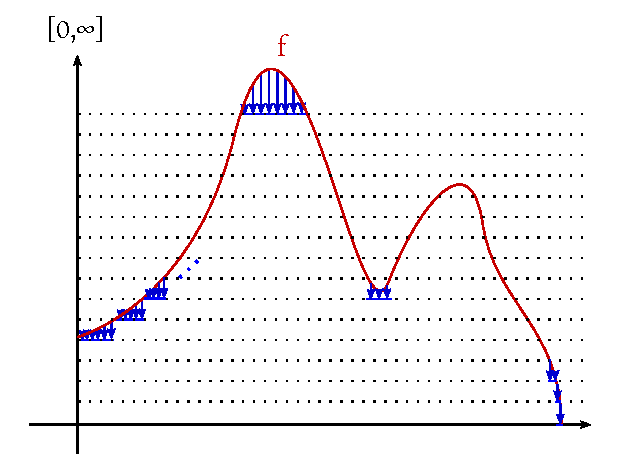
\includegraphics{img/02_lebesgue_integral.pdf}
          \caption{Illustration of the lebesgue integral}
          \label{img:lebesgue}
        \end{center}
      \end{figure}

      Let $f_n, g_n$ be simple.
      $f_n + g_n \nearrow f + g$

      \[ \int (f + g) \, d\mu \overset{\text{monotonic convergence}}{=} \lim \int (f_n + g_n) \, d\mu \]
      \[ = \lim(\int f_n \, d\mu + \int g_n \, d\mu) \overset{\text{monotonic convergence}}{=} \int f \, d\mu + \int g \, d\mu \]
  \end{enumerate}
\end{proof}

Unlike the Riemann integral, we use horizontal lines instead of vertical lines.
Thus we partition the image, not the domain.

\section{Integrable functions}

\begin{definition}
  Let $f: (X, d) \to \overline{\mathbb R}$ is measurable.
  If not $\int f^+ \, d\mu = \int f^- \, d\mu = +\infty$,
  integral exists:
  \[ \int f \, d\mu = \int f^+ \, d\mu - \int f^- \, d\mu \]
  \[ f^+ = \max\Set{f, 0} \qquad f^- = \max\Set{-f, 0} \qquad f = f^+ - f^- \qquad \Abs{f} = f^+ + f^- \]
  $f$ is called integrable, if $\int f^+ \, d\mu < \infty$ and $\int f^- \, d\mu < \infty$
  \[ \iff \int f \, d\mu \text{ exists and is finite} \]
\end{definition}

\begin{remark}[Properties]\hfill
  \begin{enumerate}
    \item $f$ is integrable $\iff \Abs{f}$ is integrable and $\Abs{\int f \, d\mu} \leq \int \Abs{f} \, d\mu$
    \item $f$, $g$ are integrable with $f \leq g$ almost everywhere wrt. $\mu$ $\implies \int f \, d\mu \leq \int g \, d\mu$
    \item $f$ is integrable, $\alpha \in \mathbb R \implies \alpha \cdot f$ is integrable and $\int (\alpha \cdot f) \, d\mu = \alpha \cdot \int f \, d\mu$
    \item $f, g$ are integrable $\implies f + g$ is integrable and $\int (f + g) \, d\mu = \int f \, d\mu + \int g \, d\mu$
  \end{enumerate}
\end{remark}

% We defined $0 \cdot \infty = 0$.  % this property is not necessary for the proof

\begin{proof}
  \begin{enumerate}
    \item $f$ is integrable
      \[ :\iff \int f^{\pm} \, d\mu < \infty \iff \underbrace{\int f^+ \, d\mu + \int f^- \, d\mu < \infty}_{\int \Abs{f} \, d\mu < \infty} \]
      \begin{align*}
        \Abs{\int f \, d\mu} &= \Abs{\int f^+ \, d\mu - \int f^- \, d\mu} \\
          &\leq \int f^+ \, d\mu + \int f^- \, d\mu \\
          &= \int \Abs{f} \, d\mu
      \end{align*}
    \item $f^+ - f^- \overset{\substack{\text{almost} \\ \text{everywhere}}}{\leq} g^+ - g^- \implies f^+ + g^- \overset{\text{a.e.}}{\leq} f^- + g^+$
      \[ \int f^+ \, d\mu + \int g^- \, d\mu = \int (f^+ + g^-) \, d\mu \leq \int \left(f^- + g^+\right) \, d\mu = \int f^- \, d\mu + \int g^+ \, d\mu \]
      \[ \int f^+ \, d\mu - \int f^- \, d\mu \leq \int g^+ \, d\mu - \int g^- \, d\mu \]
      It is important to recognize that all integrals are finite.
    \item For $\alpha = 0$, the statement is true. Consider $\alpha > 0$.
      \[ (\alpha f)^{\pm} = \alpha \cdot f^{\pm} \qquad \int \alpha f \, d\mu = \int \alpha \cdot f^+ \, d\mu - \int \alpha \cdot f^- \, d\mu = \alpha \int f^+ \, d\mu - \alpha \int f^- \, d\mu \]
      Now consider $\alpha < 0$, or more simply $\alpha = -1$ (any negative number is the product of a positive number and $-1$):
      \[ (-f)^+ = f^- (-f)^- = f^+ \qquad \dots \]
    \item $(f + g)^+ - (f + g)^- = f + g = f^+ + g^+ - (f^- + g^-)$
      \[ (f + g)^+ + f^- + g^- = (f + g)^- + f^+ + g^+ \]
      \[ \int (f + g)^+ \, d\mu + \int f^- \, d\mu + \int g^- \, d\mu = \int (f + g)^- \, d\mu + \int f^+ \, d\mu + \int g^+ \, d\mu \]
      \[ \int (f + g)^+ \, d\mu - \int (f + g)^- \, d\mu = \int f^+ \, d\mu - \int f^- \, d\mu + \int g^+ \, d\mu - \int g^- \, d\mu \]
  \end{enumerate}
\end{proof}

Riemann integral only works for $\mathbb R^n$.
The Lebesgue integral works for any measure space.

\begin{example}
  We consider the Riemann integral:
  \[ \pi = \int_{-\infty}^\infty \frac{\sin{x}}{x} \, dx \overset{\text{Riemann}}{=} \lim_{c,d\to \infty} \int_{-c}^d \frac{\sin{x}}{x} \, dx \text{ exists} \]
  If you consider $\frac{\sin{x}}{x}$ for one $\pi$, we have a positive and negative area.
  By Leibniz criterion, we have an alternating series and its limit is zero.

  We consider the Lebesgue integral:
  \[ \int_{\mathbb R} \Abs{\frac{\sin{x}}{x}} \, dx = +\infty \]
  $\frac{\sin{x}}{x}$ is not Lebesgue-integrable.
  Because in case of the Lebesgue integral, we don't consider an alternating series, but need to consider $\Abs{f}$, which is non-negative and the series does not converge.
\end{example}

\begin{theorem}[Dominated convergence theorem by Lebesgue]
  Let $f_n: (X, \mathcal A) \to \overline{\mathbb R}$ be a sequence of measurable functions.
  $f_n \to f$ pointwise [almost everywhere wrt. $\mu$]. There exists $g: (X, \mathcal A) \to [0, \infty]$ integrable [$\int g \, d\mu < \infty$].
  \[ \Abs{f_n} \leq g \text{ almost everywhere wrt. } \mu \forall n \implies \int f \, d\mu = \lim_{n\to\infty} \int f_n \, d\mu \]
\end{theorem}

\begin{proof}
  Without loss of generality, almost everywhere implies everywhere.

  \[ \Abs{f} = \lim{\Abs{f_n}} \leq g \qquad \text{ all of  them are integrable } \]
  \[ g_n = 2g - \Abs{f_n - f} \geq 0 \qquad g_n \to 2g \]
  \[ \liminf \int g_n \, d\mu \geq \int \left(\liminf g_n\right) \, d\mu \overset{g_n \to 2g}{=} \int \left(\lim g_n\right) \, d\mu = 2 \int g \, d\mu \]
  \[ \int g \, d\mu - \limsup \int \Abs{f_n - f} \, d\mu = \liminf \int g_n \, d\mu = 2\int g \, d\mu \]
  \[ \limsup\Abs{\int f_n \, d\mu - \int f \, d\mu} \leq \limsup \int \Abs{f_n - f} \, d\mu = 0 \]

  Again:
  \[ \int g_n = \left(\int 2g - \int \Abs{f_n - f}\right) \]
  \[ \implies \limsup \int g_n = \limsup \left(\int 2g - \int \Abs{f_n - f}\right) \]
  \[ = \int 2g + \limsup \left(-\int \Abs{f_n - f}\right) = \int 2g - \liminf \left(\int \Abs{f_n - f}\right) \]
\end{proof}

\dateref{2018/11/05}

\begin{Remark}[Dominated convergence theorem by Lebesgue]
  $f_n, f, g: (X, \mathcal A, \mu) \to (\mathbb R, \mathcal B_{\overline{\mathbb R}}$.
  \[ \begin{cases} f_n \to f & \mu \text{ almost everywhere} \\ \Norm{f_n} \leq g & \mu \text{ almost everywhere} \end{cases} g \geq 0, \int_{X} g \, d\mu < \infty \]
  \[ \implies \int {X} f \, dx = \lim_{n\to\infty} \int_{X} f_n \, d\mu \]
\end{Remark}

\begin{example}
  $([0, 1], \mathcal B_{[0,1]}, \lambda)$ with $f_n(x) \to 0$ and $\int_{[0,1]} f_n \, d\lambda = 1 \centernot{\implies} \int_{[0,1]} 0 \, d\mu$.
  Compare with Figure~\ref{img:exconv}.

  \begin{figure}
    \begin{center}
      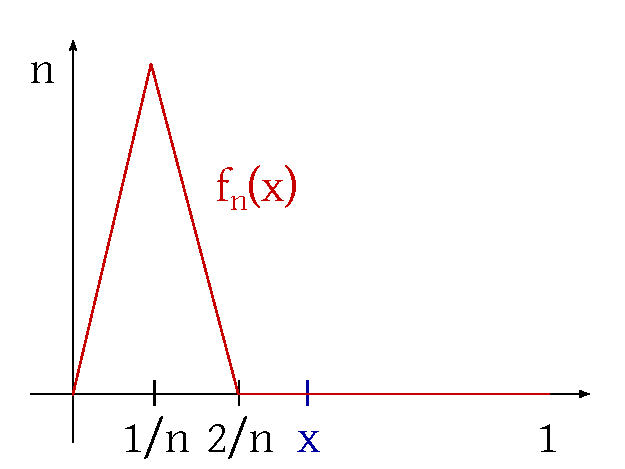
\includegraphics{img/03_convergence.pdf}
      \caption{$f_n(x)$}
      \label{img:exconv}
    \end{center}
  \end{figure}
\end{example}

The theorem of convergence is a generalization of the following theorem (based on Analysis 1 and Analysis 2 courses):

\begin{example}[Monotonic convergence]
  \[ f(x) = \sum_{n=0}^\infty a_n x^n \qquad a_n \geq 0 \]
  Convergence raidus: $R < \infty$.
  \[ x_k \nearrow R \implies f_k(x) \nearrow f(R) \]
  \[ X = \mathbb N_0, \mathcal A = \mathcal P(\mathbb N_0), \mu \]
  \enquote{counting measure}
  \[ f_k(n) = a_n x_k^n \]

  \[ f: \mathbb N_0 \to [0, \infty] \]
  \[ \int_{\mathbb N_0} f \, d\mu = \sum_{n=0}^\infty f(n) \mu(n) \]
  for $k \to \infty$: $f_k(n) \nearrow f(n) = a_n R^n$.
  By monontonic convergence, $\int f_k \, d\mu \nearrow \int f \, d\mu$.
  \[ \sum_{n=0}^\infty a_n x_k^n \nearrow \sum_{n=0}^\infty a_n R^n \]
\end{example}

\section{Lebesgue and Riemann integral}

$\lambda$ is defined on $(\overline{\mathbb R}, \mathcal B_{\overline{\mathbb R}})$.
The Lebesgue measure allows null sets. Lebesgue measure is also defined on completion of sigma algebras.
Lebesgue measure $\mathcal L$ is defined on $\sigma$-algebras of Lebesgue sets.

\begin{Remark}[One characterization of the Axiom of Choice]
  A non-empty product of non-empty sets is non-empty.
\end{Remark}
\begin{Remark}
  $\mathcal L \setminus \mathcal B \neq \emptyset$ [Axiom of Choice].
\end{Remark}

\begin{Remark}[Number representation]
  Basis $q \in \Set{2, 3, \dots}$.
  \[ x = \sum_{n=1}^\infty \frac{x_n}{q^n} \qquad x_n \in \Set{0,1,\dots,q-1} \]
  This represents a number $0 . x_1 x_2 x_3 x_4 \dots$.

  Because $0.7\overline{9} = 0.8$, there is some ambiguity between the numbers and their representation (non-bijective, two sums represent the same $x$).
\end{Remark}

\begin{Remark}[Cantor set]
  Consider $[0, 1]$. Split the interval into 3 thirds. We remove the middle third as open set.
  We consider the remaining two intervals and again extract the middle third.
  We iteratively continue this process to infinity.
  The remaining set is called Cantor set and is uncountable.

  The Cantor set $\mathcal C$ is the set of numbers in $[0,1]$ with some number representation, with respect to basis $3$, which does not contain some $1$ and has a unique number representation. Unique number representation because
  \[ \frac23 = 0.2 = 0.1\overline{2} \]
  \[ \frac13 = 0.1 = 0.0\overline{2} \qquad \frac19 = 0.01 = 0.00\overline{2} \qquad \frac29 = 0.02 = 0.01\overline{2} \]
\end{Remark}

A linear combination of Borel-measurable functions is Borel-measurable.

\begin{Remark}
  Riemann integral ($U$ are lower sums, $O$ are upper sums):
  \[ f: [a,b] \to \mathbb R \text{ bounded} \]
  \[ Z = \Set{a = x_0 < x_1 < \dots < x_k = b} \qquad \Norm{Z} = \max_{j=1,k} (x_j - x_{j-1}) \]
  \[ m_j = \inf_{x \in [x_{j-1}, x_j]} f(x) \qquad M_j = \sup_{x \in [x_{j-1}, x_j]} f(x) \]

  \[ U(Z, f) = \sum_{j=1}^k m_j(x_j - x_{j-1}) \]
  \[ g_Z = \sum_{j=1}^k m_j \mathbf{1}_{(x_{j-1}, x_j]} \text{ are both } \mathcal B\text{-measurable} \]
  \[ U(Z, f) = \sum_{j=1}^l M_j (x_j - x_{j-1}) \]
  \[ h_Z = \sum_{j=1}^k M_j \mathbf{1}_{(x_{j-1}, x_j]} \]
  \[ U(Z, f) = \int_{[a,b]} g_Z \, d\lambda \qquad O(Z, f) = \int_{[a,b]} h_Z \, d\lambda \]
\end{Remark}

\begin{theorem}
  $f$ as above (if necessary, not Borel-measurable)
  \[ C = \Set{x \in [a,b]: f \text{ continuous in } x} \quad D = \SetDef{x \in [a,b]}{f \text{ in } x \text{ is non-continuous}} \]
  \begin{enumerate}
    \item Then $C, D \in \mathcal B_{[a,b]}$, $f \cdot \mathbf{1}_C$ is Borel-measurable
    \item $f$ is Riemann integrable $\iff \lambda(D) = 0$ and
      \[ \int_a^b f(x) \, dx = \int_{[a,b]} f \cdot \mathbf{1}_C \, d\lambda \]
  \end{enumerate}
\end{theorem}

\begin{proof}
  \[ Z_n = \Set{a = x_0^{(n)} < x_1^{(n)} < \dots < x_{k(n)}^{(n)} = b} \]
  A sequence of decompositions such that
  \begin{enumerate}
    \item $Z_{n+1}$ is refinement of $Z_n$
    \item $\Norm{Z_n} \to 0$
  \end{enumerate}
  except for point $a$ (so the intervals are left-sided half-open) (you can also close the first interval of the left side)
  \[ \inf{f} = m \leq g_{Z_n} \nearrow g \leq f \leq h \swarrow h_{Z_n} \leq M = \sup{f} \]
  where $g$ and $h$ are Borel-measurable. By the dominated convergence theorem by Lebesgue,
  \[ U(Z_n, f) = \int_{[a,b]} g_{Z_n} \, d\lambda \nearrow \int_{[a,b]} g \, d\lambda \]
  \[ O(Z_n, f) = \int h_{Z_n} \, d\lambda \searrow \int_{[a,b]} h \, d\lambda \]
  $R = \SetDef{x_j^{(n)}}{n \in \mathbb N, j = 1, \dots, k(n)}$ is countable, $\lambda(R) = 0$.
\end{proof}

\begin{claim}
  For $x \in [a,b] \setminus R$, $f$ is continuous at $x \iff g(x) = h(x)$.
\end{claim}

\begin{proof}
  Let $I_n(x)$ be the interval of $Z_n$ with $x \in I_n(x)$.
  Recognize that $I_{n+1}(x) \subset I_n(x)$ and $\lambda(I_n(x)) \searrow 0$.

  \begin{align*}
    f \text{ cont. in } x
      &\iff \forall \varepsilon > 0 \exists k: f(x) - \varepsilon < f_{I_k(x)} < f(x) + \varepsilon \\
      &\iff \forall \varepsilon > 0 \forall n \geq k: f(x) - \varepsilon < f_{I_k(x)} < f(x) + \varepsilon \\
      &\iff \forall \varepsilon > 0 \exists k \forall n \geq k: f(x) - \varepsilon \leq \left. g_{Z_1} \right|_{I_n(x)} \leq \left. h_{Z_n} \right|_{I_n(x)} \leq f(x) + \varepsilon \\
      &\Rightarrow g(x) = h(x) \qquad [= f(x)]
  \end{align*}
  \enquote{$\Rightarrow$} is \enquote{$\iff$} assuming $x \not\in R$,
  so $[g < h] \subset D \subset [g < h] \cup R$ where $[g < h]$ is the Borel set.
  \[ D \setminus [g < h] \text{ is at most countable (because $R$ is countable)} \implies D \text{ Borel set}, C \text{ Borel set} \]
  \[ \lambda(D) = \lambda[g < h] \]
\end{proof}

\[ f \text{ is R-integrable } \iff \int_{[a,b]} g \, d\lambda = \int_{[a,b]} h \, d\lambda, h \geq g \]
\[ \iff \lambda[g < h] = 0 \iff \lambda(D) = 0 \]
in this case (because $g \leq f \leq h$ except in $a$).
\[ g \cdot \mathbf{1}_C = f \cdot \mathbf{1}_C \]
where $g$ and $\mathbf{1}_C$ is Borel-measurable and thus $f \cdot \mathbf{1}_C$ is Borel-measurable.
\[ \int_{[a,b]} f \cdot \mathbf{1}_C \, d\lambda = \int_{[a,b]} g \cdot \mathbf{1}_C \, d\lambda = \int_{[a,b]} g \, d\lambda = \int_a^b f(x) \, dx \]
\[ g \cdot \mathbf{1}_C = g \qquad \text{ almost everywhere wrt. } \lambda \]

\begin{example}
  \begin{enumerate}
    \item $\mathbf{1}_{\mathbb Q}$ is nowhere continuous.
      \[ \int_0^1 \mathbf{1}_{\mathbb Q}(x) \, dx \text{ does not exist} \]
      \[ \mathbf{1}_{\mathbb Q} = 0 \qquad \text{ almost everywhere wrt. } \lambda \implies \int_{[0,1]} \mathbf{1}_{\mathbb Q} \, d\lambda = 0 \]
    \item
      \[ \int_a^b \frac{\sin{x}}{x} \, dx = \int_{[a,b]} \frac{\sin{x}}{x} \, dx \]
      \[ \int_{-\infty}^\infty \frac{\sin{x}}{x} \, dx = \pi \qquad \not\exists \int_{\mathbb R} \frac{\sin{x}}{x} \, d\lambda(x) \]
  \end{enumerate}
\end{example}

\begin{theorem}[Substitution theorem]
  Let $\varphi: (X, \mathbb A, \mu) \to (X', \mathcal A')$ is measurable.
  \[ \mu_{\varphi}(A') = \mu(\varphi^{-1}(A')) \qquad A' \in \mathcal A' \qquad \text{ pushforward measure} \]
  \[ f: (X', \mathcal A') \to (\overline{\mathbb R}, \mathcal B_{\overline{\mathbb R}}) \text{ measurable} \]
  Then,
  \[ \int_{X} f \circ \varphi \, d\mu \text{ exists } \iff \int_{X'} f \, d\mu_{\varphi} \text{ exists} \]
  and in this case, they are the same.
\end{theorem}

\dateref{2018/11/12}

\begin{proof}
  \begin{enumerate}
    \item[1a.] $f = \mathbf{1}_A$, $A' \in \mathcal A' \implies f \circ \varphi = \mathbf{1}_{\varphi^{-1} A'}$
      \[ \int_{X} f\circ \varphi \, d\mu = \mu(\varphi^{-1} A') = \mu_{\varphi}(A') = \int_{X'} f \, d\mu_{\varphi} \]
    \item[1b.] $f = \sum_{k=1}^n c_k \cdot \mathbf{1}_{A'_k}$
      \[ (c_k \geq 0) \implies f \circ \varphi = \sum_{k=1}^n c_k \cdot \mathbf{1}_{\varphi^{-1} A'_k} \]
      \[ A'_k = [f = c_k] \implies \text{ statement is correct} \]
    \item[2.]
      $f \geq 0$ then $0 \leq f_n \nearrow f$ and $f_n$ is simple.
      Also $f_n \circ \varphi \nearrow f \circ \varphi$, $f_n \circ \varphi$ is simple.
      \[ \int_X f \circ \varphi \, d\mu = \lim \int_X f_n \circ \varphi \, d\mu = \lim \int_{X'} f_n \, d\mu_{\varphi} = \int_{X'} f \, d\mu_{\varphi} \]
    \item[3.]
      \[ f = f^+ - f^- \qquad f \circ \varphi = f^+ \circ \varphi - f^- \circ \varphi \]
      \[ (f \circ \varphi)^{\pm} = f^{\pm} \circ \varphi \]
      The remaining parts are obvious.
  \end{enumerate}
\end{proof}

\begin{example}
  \[ \varphi: (\mathbb R, \mathcal B) \to (\mathbb R, \mathcal B) \qquad f: (\mathbb R, \mathcal B) \to (\mathbb R, \mathcal B) \text{ $\lambda$-integrable} \]
  \[ \lambda_{\varphi}(A) = \lambda(\varphi^{-1}(A)) \]
  \[ \int_{\mathbb R} (A) = \lambda(\varphi^{-1}(A)) \]
  \[ \int_{\mathbb R} f(\varphi(x)) \, \underbrace{d\lambda(x)}_{\lambda(dx)} = \int_{\mathbb R} f(t) \, d\lambda_{\varphi}(t) \]
  by substitution $\varphi(x) = t$.
\end{example}

\begin{Remark}
  $\varphi$ is strictly monotonic. $\varphi' \neq 0$, $\varphi(\mathbb R)$.
  \[ \psi = \varphi^{-1}: \varphi(\mathbb R) \to \mathbb R \qquad \psi' \neq 0 \]

  $x = \psi(t)$
  Riemann: $dx = \psi'(t) \, dt$
  \[ \int_{-\infty}^{\infty} f(\varphi(x)) \, dx = \left.\int_c^d f(t)\right|_{\psi'(t)} \]

  \[ \lim \frac{\varphi(x + h) - \varphi(\lambda)}{x} \]

  TODO


\end{Remark}

% previously: Sigma algebras and measures
\section{Construction of measures}

\subsection{Dynkin systems, Uniqueness theorem}
\index{Dynkin system}
\index{$\pi$-system}
\begin{definition}
  $\mathcal D \subset \mathcal p(X)$ is called \emph{Dynkin system} or $\pi$-system, if
  \begin{enumerate}
    \item $X \in \mathcal D$
    \item $A \in \mathcal D \implies A^C \in \mathcal D$
    \item $A_n \in \mathcal D$ ($n \in \mathbb N$) is pairwise disjoint then $\bigcupdot_n A_n \in \mathcal D$
  \end{enumerate}
\end{definition}
$\mathcal D$ is a non-empty family of subsets of $X$ that is closed under finite intersections.

Obviously,
\begin{enumerate}
  \item Every $\sigma$-algebra is a Dynkin system
  \item $\varepsilon \subset \mathcal P(X)$, $D(\varepsilon)$ is generated $D$-system
    \[ \implies \varepsilon \subset \mathcal D(\varepsilon) \subset \sigma(\varepsilon) \]
\end{enumerate}

The intersection of Dynkin systems is a Dynkin system

\begin{lemma}
  $\mathcal D$ as Dynkin system is a $\sigma$-algebra $\iff$ closed under intersection ($A, B \in \mathcal D \implies A \cap B \in \mathcal D$)
\end{lemma}

\begin{proof}
  \begin{description}
    \item[$\implies$] is immediate
    \item[$\impliedby$]
      Let $A_n \in \mathcal D$ ($n \in \mathbb N$)
      \[ B_1 = A_1 \in \mathcal D, B_2 = A_2 \setminus (B_1 \cap A_2) = \underbrace{A_2}_{\in \mathcal D} \cap \underbrace{(B_1 \cap A_2)^C}_{\in \mathcal D} \in \mathcal D \]
      \[ B_n = A_n \setminus \underbrace{\left(\underbrace{\bigcupdot_{i=1}^{n-1} B_i}_{\in \mathcal D} \cap \underbrace{A_n}_{\in \mathcal D}\right)}_{\in \mathcal D} \]
      \[ \bigcup_{n=1}^\infty A_n = \bigcupdot_{n=1}^\infty B_n \in \mathcal D \]
  \end{description}
\end{proof}

\begin{lemma}
  \label{lamme:3-2}
  Let $\varepsilon \subset \mathcal P(X)$ is closed under intersection $\implies \mathcal D(\varepsilon) = \sigma(\varepsilon)$
\end{lemma}

\begin{proof}[Good set principle]
  We have to show $\mathcal D(\varepsilon)$ is closed under intersection. Let $D \in \mathcal D(\varepsilon)$.
  \[ \mathcal D_D \coloneqq \SetDef{A \subset X}{A \cap D \subset \mathcal D(\varepsilon)} \text{ is a $\mathcal D$-system?} \]
  \begin{enumerate}
    \item Trivial
    \item $A \in \mathcal D_D$. $A^C \cap D = \dots = \left((A \cap D) \dot\cup D^C\right)^C \in \mathcal D(\varepsilon)$
    \item Trivial
  \end{enumerate}
  Yes, it is. Especially:
  \[ E \in \underbrace{\varepsilon}_{\subset \mathcal D(\varepsilon)} \qquad A \in \varepsilon \implies A \cap E \in \underbrace{\varepsilon}_{\subset \mathcal D(\varepsilon)} \qquad A \in \mathcal D_E \]
  \[ \implies \varepsilon \subset \mathcal D_E \implies \mathcal D(\varepsilon) \subset \mathcal D_E \forall E \in \varepsilon \]
  \[ D \in \mathcal D(\varepsilon) \implies D \in \mathcal D_E \implies E \cap D \in \mathcal D(\varepsilon) \implies E \in \mathcal D_D \forall E \in \varepsilon \]
  \[ \varepsilon \subset \mathcal D_D, \text{ so } \mathcal D(\varepsilon) \subset \mathcal D_D \implies D' \cap D \in \mathcal D(\varepsilon) \forall D' \in \mathcal D(\varepsilon) \text{ is true } \forall D \in \mathcal D(\varepsilon) \]
\end{proof}

\begin{theorem}[Uniqueness theorem]
  $\mathcal A = \sigma(\varepsilon)$, $\varepsilon$ is closed under intersection. $\mu$ and $\nu$ are measure on $\mathcal A$.
  \begin{enumerate}
    \item $\left.\mu\right|_{\varepsilon} = \left.\nu\right|_{\varepsilon}$
    \item $\mu(X) = \nu(X) < \infty$ or $\varepsilon \ni E_n \nearrow X, \mu(E_n) = \nu(E_n) < \infty \forall n$
  \end{enumerate}
  Then $\mu = \nu$ on $\mathcal A$.
\end{theorem}

\begin{proof}
  Let $E \in \varepsilon$ with $\mu(E) = \nu(E) < \infty$ and
  $S_E = \SetDef{D \in \mathcal A}{\mu(D \cap E) = \nu(D \cap E)} \subset \mathcal A$
  \begin{itemize}
    \item $\varepsilon \in S_E$ (because of closure under intersection)
    \item $S_E$ is a Dynkin system
      \begin{enumerate}
        \item trivial
        \item $D \in S_E$, $E = (D \cap E) \dot\cup (D^C \cap E)$
          \begin{align*}
            \mu(E) = \mu(D \cap E) + \mu(D^C \cap E):
              &\: \mu(D^C \cap E) = \mu(E) - \mu(D \cap E) \\
              & \nu(D^C \cap E) = \nu(E) - \nu(D \cap E)
          \end{align*}
          \[ \mu(D^C \cap E) = \nu(D^C \cap E), D^C \in S_E \]
        \item $D_n \in S_E$ pairwise disjoint
          \[
            \mu\left(\left(\bigcup_{n=1}^\infty D_n\right) \cap E\right)
              = \sum_{n=1}^\infty \mu\left(D_n \cap E\right)
              = \sum_{n=1}^\infty \nu(D_n \cap E)
          \] \[
              = \nu\left(\left(\bigcupdot_{n=1}^\infty D_n\right) \cap E\right)
            \implies \bigcupdot_{n=1}^\infty D_n \in S_E
          \]
      \end{enumerate}
      \[
        \varepsilon \subset \mathcal A = \mathcal D(\varepsilon) \subset S_E
      \] \[
        \mu(A \cap E) = \nu(A \cap E) \forall A \in \mathcal A
      \]
      \begin{enumerate}
        \item $E = X$: $\mu = \nu$
        \item $\mu(A \cap E_n) \nearrow \mu(A \cap X)$ \\
          $\nu(A \cap E_n) \nearrow \nu(A \cap X) \forall A \in \mathcal A$
          \[ \implies \mu = \nu \]
      \end{enumerate}
  \end{itemize}
\end{proof}

\dateref{2018/11/19}

\subsection{Outer measure and extension theorem}
\begin{definition}[Outer measure]
  \index{Outer measure}
  $\eta: P(X) \to [0, \infty]$ is called \emph{outer measure} if
  \begin{enumerate}
    \item $\eta(\emptyset) = 0$
    \item $\sigma$-additivity
  \end{enumerate}
  \[ \implies A \subset \bigcup_{n=1}^\infty A_n \implies \eta(A) \leq \sum_{n=1}^\infty \eta(A_n) \]

  $A \subset X$ is called $\eta$-measurable if $\forall C \subset X: \eta(C \cap A) + \eta(C \cap A^C) = \eta(C)$.

  Is not a measure.
\end{definition}

\begin{Remark}
  Third property: $A \subset B \implies \eta(A) \leq \eta(B)$
\end{Remark}

\begin{theorem}[Carathéodory]
  $A_\eta = \SetDef{A \subset \mathcal P(X)}{A \text{ measurable}}$ is a $\sigma$-algebra and $\left.\eta\right|_{\mathcal A_{\eta}}$ is a measure, $(X, \mathcal A_\eta, \eta)$ is complete.
\end{theorem}

\begin{proof}
  \[ \forall C: \eta(C \cap X) + \underbrace{\eta(C \cap \emptyset)}_{\sigma(i)} = \eta(C) \implies X \in \mathcal A_\eta \]
  Thus, the first statement follows. For the second property, we have:

  $A$ is measurable, then $A^C$ is measurable.
  By finite union and additivity:
  \[ A_1, A_2 \in \mathcal A_\eta \implies \forall C \in \mathcal P(X) \]

  \begin{align*}
    \eta(C) &= \eta(C \cap A_1) + \eta(C \cap A_1^C) \\
      &= \eta(C \cap A_1) + \eta\left((C \cap A_1^C) \cap A_2\right) + \eta\left((C \cap A_1^C) \cap A_2^C\right) \\
      &= \eta\left(C \cap (A_1 \cup A_2) \cap A_1\right) + \eta(C \cap (A_1 \cup A_2) \cap A_1^C) + \eta(C \cap (A_1 \cup A_2)^C) \\
      &\overset{A_1 \text{ measurable}}{=} \eta\left(C \cap (A_1 \cup A_2)\right) + \eta(C \cap (A_1 \cup A_2)^C) \\
      &\implies A_1 \cup A_2 \text{ measurable}
  \end{align*}
  If $A_1 \cap A_2 = \emptyset$
  \begin{align*}
    \eta(C \cap (A_1 \cup A_2) \cap A_1) + \mu(C \cap (A_1 \cup A_2) \cap A_1^C)
      &= \eta(C \cap A_1) + \eta(C \cap A_2)
  \end{align*}
  Especially, $C = X$, $\eta(A_1 \dotcup A_2) = \eta(A_1) + \eta(A_2)$.

  Also $A_1, A_2 \in \mathcal A_\eta \implies A_1 \cap A_2 = (A_1^C \cup A_2^C)^C \in \mathcal A_\eta$.

  $\sigma$:
  $A_n \in \mathcal A_\eta$ ($n \in \mathbb N$) with $p_n$ disjoint.
  $\bigcup_{n=1}^N A_n \in \mathcal A_\eta$. Let $C \subset X$.
  \begin{align*}
    \eta(C) &= \eta\left(C \cap \bigcup_{n=1}^N A_n\right) + \eta\left(C \cap \left(\bigcup_{n=1}^N A_n\right)^C\right) \\
      &\geq \underbrace{\sum_{n=1}^N \eta(C \cap A_n)}_{\forall N} + \eta\left(C \cap \left(\bigcup_{n=1}^\infty A_n\right)^C\right) \\
      &\overset{\text{by $\sigma$-subadd.}}{\geq} \eta\left(C \cap \bigcupdot_{n=1}^\infty A_n\right) + \eta\left(C \cap \left(\bigcup_{n=1}^\infty A_n\right)^C\right) \\
      &\implies \bigcupdot_{n=1}^\infty A_n \text{measurable}, \eta\left(\bigcupdot_{n=1}^\infty \eta(A_n)\right) + 0
  \end{align*}
  We know: $\mathcal A_\eta$ is a Dynkin system and closed under intersection (thus, a $\sigma$-algebra).
  $\eta$ is $\sigma$-additive on $\mathcal A_\eta$.

  Completeness is obvious.
\end{proof}

\begin{theorem}[Carathéodory's extension theorem]
  Let $\varepsilon \subset \mathcal P(X)$ be the generator of $\mathcal A$.
  Let $\mu: \varepsilon \to [0, \infty]$ be a set functions. $A \subset X$.
  \[ \mu^*(A) = \inf\SetDef{\sum_{n=1}^\infty \mu(E_1)}{E_1 \in \varepsilon, A \subset \bigcup_{n=1}^\infty E_1} \]
  \begin{enumerate}
    \item $\mu^*$ is an outer measure $\iff \mu^*(\emptyset) = 0$ (especially true, if $\, \emptyset \in \varepsilon$ and $\mu(\emptyset) = 0$)
    \item If $\mu^*(\emptyset) = 0$, $\varepsilon \subset \mathcal A_{\mu^*} \iff \mu^*(D \cap E) + \mu^*(D \cap E^C) \leq \mu(D) \forall D, E \in \varepsilon$
    \item If the first two properties are satisfied, then $\left.\mu^*\right|_\varepsilon = \mu$ iff $\mu^*(E) \geq \mu(E) \forall E \in \varepsilon$, so $\mu(E) \leq \sum_{n=1}^\infty \mu(E_n)$ if $E_n \in \varepsilon$ and $E \subset \bigcup_{n=1}^\infty E_n$
  \end{enumerate}
\end{theorem}

$\mu^*$ is $\sigma$-subadditive in every case.

$\forall \delta > 0 \exists E_n \in \varepsilon: \sum \mu(E_n) < \delta$ \\
$E \subset E \cup \bigcup_n E_n$ \\
$\mu^*(E) \leq \mu(E) + \sum_n \mu(E_n) \leq \mu(E) + \delta$. \\
Thus, $\mu^*(\emptyset) = 0 \implies \mu^*(E) \leq \mu(E) \forall E \in \varepsilon$

\begin{proof}
  \begin{enumerate}
    \item Direction $\implies$ is immediate. \\
      For direction $\impliedby$, we need to show $\sigma$-subadditivity.

      \[ A, A_n \in X, A \subset \bigcup_{n=1}^\infty A_n \]
      \[ \mu^*(A_n) = \inf\SetDef{\sum_{m=1}^\infty \mu(E_{m,n})}{E_{m,n} \in \varepsilon, A_n \subset \bigcup_{m=1}^\infty E_{m,n}} \]
      $\delta > 0: \exists E_{m,n} \in \varepsilon: \mu^*(A_n) + \frac{\delta}{2^n} \geq \sum_{m=1}^\infty \mu(E_{m,n}) \geq \mu^*(A_n)$
      \[ A \subset \bigcup_{n=1}^\infty A_n \subset \bigcup_{n=1}^\infty \bigcup_{m=1}^\infty E_{m,n} \]
      \begin{align*}
        \mu^*(A) &\leq \sum_{n=1}^\infty \sum_{m=1}^\infty \mu\left(E_{m,n}\right) \\
          &\leq \sum_{n=1}^\infty \left(\mu^*(A_n) + \frac{\delta}{2^n}\right) \\
          &= \sum_{n=1}^\infty \mu^*(A_n) + \delta \forall \delta > 0 \\
          &\implies \mu^*(A) \leq \sum_{n=1}^\infty \mu^*(A_n)
      \end{align*}
    \item Direction $\implies$ is immediate. \\
      For direction $\impliedby$, let $E \in \varepsilon$. Show that $E$ is measurable with respect to $\mu^*$.

      Let $C \subset X$ be arbitrary. $D_n \in \varepsilon$ such that $C \subset \bigcup_{n=1}^\infty D_n$ and $\mu^*(C) + \delta \geq \sum_{n=1}^\infty \mu(D_n) \geq \mu^*(C)$
      \begin{align*}
        \mu^*(C) &\leq \mu^*(C \cap E) + \mu^*(C \cap E^C) \\
          &\leq \sum_{n=1}^\infty \left(\mu^*(D_n \cap E) + \mu^*(D_n \cap E)\right) \\
          &\overset!\leq \sum_{n=1}^\infty \mu(D_n) \leq \mu^*(C) + \delta \forall \delta > 0
      \end{align*}
      So, $\mu^*(C \cap E) + \mu^*(C \cap E^C) = \mu^*(C)$ where $E$ is measurable.
  \end{enumerate}
\end{proof}

\begin{theorem}
  Let $\varepsilon$ be a semiring. $\mu: \varepsilon \to [0, \infty]$.
  \begin{enumerate}
    \item $\mu(\emptyset) = 0$
    \item $X \in \varepsilon$ and $\mu(X) < \infty$ or $X = \bigcup_n E_n$, $E_n \in \varepsilon, \mu(E_n) < \infty$
    \item $\mu$ is $\sigma$-additive on $\varepsilon \implies$ unique extension on $\sigma(\varepsilon)$
  \end{enumerate}
  $\varepsilon$ is a semiring over $X$, if
  \begin{enumerate}
    \item $\emptyset \in \varepsilon$
    \item $D, E \in \varepsilon \implies D \cap E \in \varepsilon$
    \item $D \setminus E = C_1 \dot\cup \dots \dot\cup C_k, C_k \in \varepsilon$
  \end{enumerate}
  $\mu: \varepsilon \to [0, \infty]$ is $\sigma$-additive on $\varepsilon$.

  where $\mu(\emptyset) = 0$, $\mu\left(\bigcupdot_n E_n\right) = \sum_n \mu(E_n)$
  if $\bigcupdot_{n} E_n \in \varepsilon$
\end{theorem}

\[ X = \bigcup_n E_n \qquad E_n \in \varepsilon \qquad \mu(E_n) < \infty \]
Thus, the theorem is applicable, so $\mu$ has a unique extension for measure
to $\mathcal A_{\mu^*} \supset \mathcal A \supset \varepsilon$. $\mathcal A_{\mu^*}$ complete.

\begin{proof}
  \begin{itemize}
    \item $\mu$ also finitely additive on $\varepsilon$.
    \item $D, E \subset \varepsilon$. $E \subset D \implies D \setminus E = C_1 \dot\cup \dots \dot\cup C_k$. $D = E \dot\cup C_1 \dot\cup \dots \dot\cup C_k$
      \[ \mu(D) = \mu(E) + \sum \mu(C_j) \geq \mu(E) \]
  \end{itemize}
  \begin{enumerate}
    \item Immediate.
    \item $D, E \in \varepsilon$. $D \cap E \in \varepsilon. D \cap E^C = C_1 \dot\cup \dots \dot\cup C_k$ with $C_j \in \varepsilon$. $D = (D \cap E) \dot\cup C_1 \dot\cup \dots \dot\cup C_k$. $\mu^*(D \cap E) + \mu^*(D \cap E^C) \leq \mu(D \cap E) + \sum_{j=1}^k \mu(C_j) = \mu(D)$.
    \item $E , E_n \in \varepsilon: E \subset \bigcup_{n=1}^\infty E_n$. $E = \bigcup_{n=1}^\infty \underbrace{(E_n \cap E)}_{\in \varepsilon}$ it suffices to show that $\mu(E) \leq \sum_n \mu(E_n \cap E)$.
    Without loss of generality, $E = \bigcup_{n=0}^\infty E_n$. $D_1 = E_1$, $D_2 = E_2 \cap E_1^C = C_{2,1} \dot\cup \dots \dot\cup C_{2,k_2}$. $D_n = E_n \cap E^C_{n-1} \cap \dots \cap E_1^C = C_{n,1} \dot\cup C_{n,2} \dot\cup \dots \dot\cup C_{n,k_n}$. $C_{n,j} \in \varepsilon$.
    \[ E = \bigcup_{n=1}^\infty E_n = \bigcupdot_{n=1}^\infty D_n = \bigcupdot_{n=1}^\infty \bigcupdot_{j=1}^{k_n} C_{n,j} \]
    \[ \mu(E) = \sum_{n=1}^\infty \underbrace{\sum_{j=1}^{k_n} \mu(C_{n,j})}_{\leq \mu(E_n)} \leq \sum_n \mu(E_n) \]
  \end{enumerate}
\end{proof}

\subsection{Regular measures}

\index{Outer regular measure}
\begin{definition}
  Let $(X, \mathcal A, \mu)$ is a measurable space. Let $\varepsilon$ be a generator of $\mathcal A$.
  $\mu$ is called \emph{outer regular} with respect to $\varepsilon$,
  if $\mu = \mu^*$ on $d$ where $\mu^*$ is defined like
  \[ \mu^*(A) = \inf\SetDef{\sum_{n=1}^\infty \mu(E_1)}{E_1 \in \varepsilon, A \subset \bigcup_{n=1}^\infty E_1} \]
  \dt{$\mu$ is regulär von außen}
\end{definition}

\begin{theorem}
  Let $\varepsilon$ be a generator closed under intersection. Let $\emptyset \in \varepsilon$.
  Let $\mu$ be a measure on $\mathcal A = \sigma(\varepsilon)$, $\sigma$-finite with respect to $\varepsilon$.
  \[ \mu^*(A) \coloneqq \inf\SetDef{\sum_{n=1}^\infty \mu(E_1)}{E_1 \in \varepsilon, A \subset \bigcup_{n=1}^\infty E_1} \]
  Then $\mu = \mu^*$ on $\mathcal A$ ($\mu$ is outer regular) $\iff$
  \[ \mu(D \cap E^C) = \mu^*(D \cap E^C) \forall D, E \in \varepsilon \]
\end{theorem}

\begin{proof}
  \begin{enumerate}
    \item trivial
    \item
      $\mu(E) \geq \mu^*(E)$ with $E \in \varepsilon$.
      By (3), we have $\mu(E) \leq \mu^*(E)$.
      $\mu(E) = \mu^*(E)$ on $\varepsilon$.
      $D, E \in \varepsilon: \mu^*(D \cap E) + \mu^*(D \cap E^C) = \mu(D \cap E) + \mu(D \cap E^C) = \mu(D)$.
      Thus $E \subseteq D$.

      \begin{Remark}
        \[ D \cap E^C = D \cap (E \cap D)^C \]
        \[ \mu^*(D \cap E) + \mu^*(D \cap E^C) = \mu(D \cap E) + \mu^*(\underbrace{D}_{\in \varepsilon} \cap (\underbrace{E \cap D}_{\in \varepsilon})^C) \]
        \[ = \mu(D \cap E) + \mu(D \cap (E \cap D)^C) = \mu(D \cap E) + \mu(D \cap E^C) = \mu(D) \]
      \end{Remark}
    \item trivial
  \end{enumerate}
\end{proof}

\begin{theorem}
  Let $X$ be a metric space. $\varepsilon = \Set{\text{open sets}}$.
  $\mathcal B_{X} = \sigma(\varepsilon)$ is a Borel-$\sigma$-algebra.
  $\mu$ is a $\sigma$-finite measure on $(X, \mathcal B_{X})$.
  \begin{align*}
    \mu(B) &= \inf\SetDef{\mu(O)}{O \supset B \text{ open}} \\
           &= \sup\SetDef{\mu(A)}{A \subset B \text{ closed}}
  \end{align*}
\end{theorem}

\begin{proof}
  Without loss of generality: $\mu(X) < \infty$.
  \[ B \subset O = \bigcup_{n=1}^\infty E_n \text{ open} \]
  \[ \mu(B) \leq \mu(O) \leq \sum_{n=1}^\infty \mu(E_n) \]
  In combination,
  \[ \mu^*(B) = \inf\SetDef{\mu(O)}{O \supset B} \]
  $\varepsilon$ is closed under intersection. $\emptyset \in \varepsilon$.
  $A = E^C$ is closed. Is $E \subset D$ open? $\mu^*(D \cap E^C) = \mu(D \cap E^C)$.
  $A_n = \SetDef{x}{d(x, A) < \frac1n}$ open, $A_n \searrow A$
  where $\searrow$ denotes a monotonically decreasing sequence converging from the LHS to the RHS.
  \[ D \cap E^C = D \cap A \swarrow \underbrace{D \cap A_n}_{\in \varepsilon, \text{ open}} \]
  \[ \mu(D \cap A_n) \searrow \mu(D \cap A) \]
  Like above: In $\varepsilon$, we have $\mu = \mu^*$.
  \[ \underbrace{\mu^*(D \cap A_n)}_{\geq \mu^*(D \cap E^C)} = \underbrace{\mu(D \cap A_n)}_{\to \mu(D \cap E^C)} \]
  Thus, $\mu^*(D \cap E^C) \leq \mu(D \cap E^C)$.
  In contrast, we already have $\mu$ on entire $\sigma$-algebra. So $\forall B \in \mathcal B: \mu(B) \leq \mu(O) \forall O \supset B$ open. $\mu(B) \leq \mu^*(B)$ and therefore $\mu^*(D \cap E^C) \leq \mu(D \cap E^C) \leq \mu^*(D \cap E^C)$.
  So $\mu = \mu^*$.
\end{proof}

\subsection{Product measures and Fubini's Theorem}

\dateref{2018/12/03}

Let $(X, \mathcal A, \mu)$ and $(Y, \mathcal B, \nu)$ be measure space.
Let $\mu$ and $\nu$ be $\sigma$-finite.
$A \otimes B = \sigma(\varepsilon)$. $\varepsilon = \Set{A \times B: A \in \mathcal A, B \in \mathcal B}$.
$\mu \otimes \nu (A \times B) = \mu(A) \nu(B)$.

\begin{definition}
  \label{def:fub}
  Let $C \in \mathcal A \otimes \mathcal B$. $C_x = \SetDef{y \in Y}{(x, y) \in C}$ with $x \in X$.
  $C^Y = \SetDef{x \in X}{(x, y) \in C}$.

  \begin{figure}[!ht]
    \begin{center}
      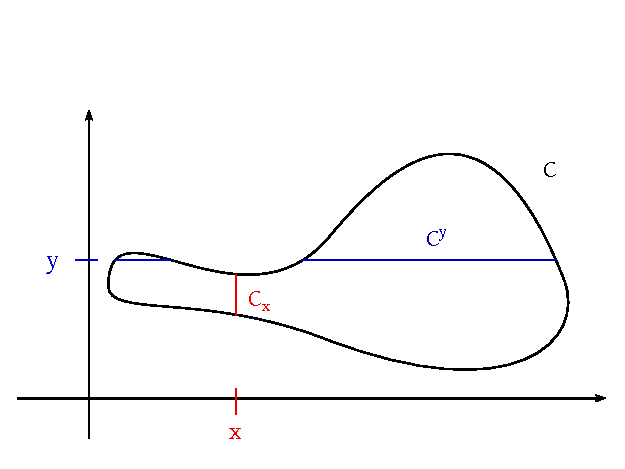
\includegraphics{img/fubini_theorem.pdf}
      \caption{Setting in Definition~\ref{def:fub}}
      \label{img:fubini}
    \end{center}
  \end{figure}

  \[ f: X \times Y \to \overline{\mathbb R} \]
  \[ f_x: Y \to \overline{\mathbb R} \qquad f_x(y) = f(x, y) \]
  \[ f^y: X \to \overline{\mathbb R} \qquad f^y(x) = f(x, y) \]
\end{definition}

\begin{theorem}
  \[ C \in \mathcal A \otimes \mathcal B \implies C_x \in \mathcal B \forall x \in X, C^y \in \mathcal A \forall y \in Y \]
  \[ f \text{ measurable } \implies f_x, f^y \text{ measurable } \forall x \in X, y \in Y \]
\end{theorem}

\begin{proof}
  \[ \mathcal D = \SetDef{C \in \mathcal A \otimes \mathcal B}{C_x \in \mathcal B \forall x \in X} \]
  \[ \varepsilon \subset \mathcal D (\text{closed under intersection}) \qquad (A \times B)_{x} = \begin{cases} B & x \in A \\ \emptyset & x \not\in A \end{cases} \]
  \[ (C_x)^C = (C^c)_x \text{ so } C \in \mathcal D \implies C^C \in \mathcal D \]
  \[ C_1, C_2, \dots \in \mathcal D, \text{ pairwise disjoint } \implies \left(\bigcup_{n}^+ C_n\right)_x = \bigcup_{n}^+ \underbrace{C_{n,x}}_{\in \mathcal B} \in \mathcal B \]
  \[ \mathcal D \text{ Dynkin } \implies \mathcal D = \mathcal A \otimes \mathcal B \]

  \[ f \geq 0: f_n = \sum_k c_{n,k} \mathbf{1}_{c_{n,k}} \]
  \[ C_{n,k} \in \mathcal A \otimes \mathcal B \text{ for fixed } n \]
  pairwise disjoint
  \[ f_n \nearrow f \qquad f_{n,x} \nearrow f_x \]
  \[ f_{n,x} = \sum_k c_{n,k} \underbrace{\mathbf{1}_{(C_{n,k})x}}_{\in \mathcal B} \]
  $\mathcal B$-measurable $\implies f_x$ $\mathcal B$-measurable.
\end{proof}

\begin{Remark}
  In general, $f = f^+ - f^-$, $f^{\pm}$ measurable, $f_x = f_x^+ - f_x^-$ ($f_x^+$ and $f_x^-$ are measurable).
\end{Remark}

\begin{definition}[Definition and theorem]
  There exists exactly one measure $g$ on $\mathcal A \otimes \mathcal B$ such that $g(A \times B) = \mu(A) \nu(B) \forall A \in \mathcal A, B \in \mathcal B$ and
  \[ g(C) = \int_X \nu(C_x) \, d\mu(x) = \int_Y \nu(C^y) \, d\nu(y) \forall C \in \mathcal A \otimes \mathcal B \]
\end{definition}

\begin{Remark}
  This implies that $x \mapsto \nu(C_x)$ is measurable and $y \mapsto \nu(C^y)$ is measurable.
\end{Remark}

\begin{proof}
  The uniqueness follows from the uniqueness theorem.

  What about existence? Without loss of generality, $\mu(X) < \infty$ and $\nu(Y) < \infty$.
  \[
    \mathcal D = \SetDef{C \in \mathcal A \otimes \mathcal B}%
      {x \mapsto \nu(C_x), y \mapsto \mu(C^y) \text{ measurable }\forall x, y \text{ and G}}
  \]
  where $G$ means that the following property (from before) is true:
  \[ g(C) = \int_X \nu(C_x) \, d\mu(x) = \int_Y \nu(C^y) \, d\nu(y) \forall C \in \mathcal A \otimes \mathcal B \]

  \begin{align*}
    \varepsilon \subset \mathcal D:
      & \nu((A \times B)_x) = \nu(B) \mathbf{1}_A(x) \\
      & \mu((A \times B)^y) = \mu(A) \mathbf{1}_B(x)
  \end{align*}

  \[ \int_{X} \nu((A \times B)_x) \, d\mu(x) = \nu(B) \mu(A) \]
  \[ \int_{Y} \mu((A \times B)^y) \, d\nu(y) = \mu(A) \nu(B) \]

  \[ C \in \mathcal D \qquad \nu\left((C^C)_x\right) = \nu(C_x^C) = \underbrace{\nu(Y)}_{\text{measurable}} - \nu(C_x) \]
  \[ \mu((C^C)^y) = \underbrace{\mu(X) - \mu(C^y)}_{\text{measurable}} \]
  \begin{align*}
    \int_X \nu((C^C)_x) \, d\mu(x)
      &= \int_X \left(\nu(y) - \nu(C_x)\right) \, d\mu(x) = \mu(X) \nu(Y) - \int_X \nu(C_x) \, d\mu(x) \\
      &= \nu(Y) \mu(X) - \int_Y \mu(C^y) \, d\nu(y) \\
      &= \dots \\
      &\implies C^C \in \mathcal D]
  \end{align*}

  $C_1 \in \mathcal D$ is pairwise disjoint.
  \[ \nu\left(\left(\bigcup_n^+ C_n\right)_x\right) = \sum_n \nu(C_{n,x}) \qquad \mu\left(\left(\bigcup_n^+ C_n\right)^y\right) = \sum_n \mu(C_n^y) \]
  where the elements of both inner parentheses are measurable as function of $x$ and $y$ respectively.
  \begin{align*}
    \int \nu\left(\left(\bigcup_n^+ C_1\right)_x\right) \, d\mu(x)
      &= \sum_n \int_X \nu(C_{n,x}) \, d\mu(x) \\
      &\underbrace{=}_{C_n \in \mathcal D} \sum_n \int_Y \mu(C_n^y) \, d\nu(y) \\
      &= \int \mu\left(\left(\bigcup_n^+ C_n\right)^y\right) \nu(dy) \\
      &\implies \bigcup^+ C_n \in \mathcal D, \mathcal D \text{ Dynkin system } \\
      &\implies \mathcal D = \mathcal A \times \mathcal B
  \end{align*}
  Furthermore $\rho(C) \coloneqq \int_X \nu(C_x) \, d\mu(x)$ \emph{is} a measure with $\rho(A \times B) = \mu(A) \nu(B)$.
\end{proof}

\begin{Remark}
  From now on: $g \longleftrightarrow \mu \otimes \nu$
\end{Remark}

\begin{theorem}[Fubini-Tonelli Theorem]
  Let $f: X \times Y \to [0, \infty]$ be measurable. Then
  \[ \int_{X \times Y} f \, d\mu \times \nu = \int_X \left[\int_Y f_X \, d\nu\right] \, d\mu(x) = \int_Y \left[\int_X f^Y \, d\mu \right] \, d\nu(x) \]
\end{theorem}

Equivalently, we can formulate this theorem as
\[ \int_X \left[\int_Y f(x, y) \, d\nu(y)\right]\, d\mu(x) = \int_Y \left[\int_X f(x,y) \, d\mu(x)\right] \, d\nu(y) \]

\begin{remark}
  This theorem implies that $x \mapsto \int_Y f_X \, d\nu$ and $y \mapsto \int_X f^Y \, d\mu$ are measurable.
\end{remark}

\begin{proof}
  \begin{enumerate}
    \item $f = \mathbf{1}_C$ with $C \in \mathcal A \otimes \mathcal B$ \\
      corresponds to the previous theorem $\qquad C_k \in \mathcal A \otimes \mathcal B$
    \item $f = \sum_{k=1}^N c_k \mathbf{1}_{C_k}$ is pairwise disjoint, $c_k \geq 0$ \\
      follows by linearity of the integral

      \[ \int_Y f_x \, d\nu = \sum_k c_k \nu(C_{k,x}) \]
      \begin{align*}
        \int_X \left(\int_Y f_X \, d\nu\right) \, d\mu(x)
          &= \sum_k c_k \int \nu(C_{k,x}) \, d\mu(x) \\
          &= \sum_k c_k \mu \otimes \nu(C_k) = \int_{X \times Y} f \, d\mu \otimes \nu = \text{ vice versa}
      \end{align*}
    \item $0 \leq f_n \nearrow f$. $f_n$ is simple. Monotone convergence.
  \end{enumerate}
\end{proof}

\begin{theorem}[Fubini]
  \[ f: X \times Y \to \mathbb R \text{ measurable} \]
  Then the following statements are equivalent:
  \begin{enumerate}
    \item $\int_{X \otimes Y} \Abs{f} \, d\mu \otimes \nu < \infty$
    \item $\int_{X} \left[ \int_Y \Abs{f_X} \, d\nu \right] \, d\mu(x) < \infty$
    \item $\int_{Y} \left[ \int_{X} \Abs{f^Y} \, d\mu \right] \, d\nu(y) < \infty$
  \end{enumerate}
  Especially, $\Abs{f}_X = \Abs{f_X}$. Fubini's theorem is obvious due to Fubini-Tonelli's theorem.
\end{theorem}

\begin{proof}
  and then
  \begin{align*}
    \int f \, d\mu \otimes \nu
      &= \int_X \left[ \int_Y \hat{f}(x, y) \, d\nu(y) \right] \, d\mu(x) \\
      &= \int_Y \left[ \int_X \hat{\hat{f}}(x, y) \, d\mu(x) \right] \, d\nu(y) \\
  \end{align*}
\end{proof}

\begin{remark}[Reminder]
  $f$ is integrable iff $\int f^+ < \infty$ and $\int f^- < \infty$
  and then $\int f = \int f^+ - \int f^-$, $\int \Abs{f} = \int f^+ + \int f^-$.
  Especially: $\Abs{\int f} \leq \int \Abs{f}$
\end{remark}

\begin{proof}
  \[ \int \left[\int f_x^\pm \, d\nu\right] \, d\mu(x) < \infty \implies \int_Y f_x^\pm \, d\nu < \infty \quad \mu \text{ almost everywhere} \]
  \[ A_0 = \SetDef{x}{\int_Y \Abs{f_X} \, d\nu = \infty} \in \mathcal A \qquad \mu(A_0) = 0 \]
  \[ B_0 = \SetDef{y}{\int_X \Abs{f^Y} \, d\mu = \infty} \in \mathcal B \qquad \nu(B_0) = 0 \]
  \[ C_0 = \left(A_0 \otimes Y\right) \cup \left(X \times B_0\right) \qquad \mu \otimes \nu(C_0) = 0 \]
  $\mu \otimes \nu(C_0) = 0$
  \[ f = \hat{\hat{f}} = f \cdot \mathbf{1}_{X \times Y: C_0} \]
  $\mu \otimes \nu$ almost everywhere.

  \begin{align*}
    \hat{f}_x &= f_x  \qquad \nu\text{ almost everywhere} \\
    \hat{\hat{f}}^y &= f^y  \qquad \mu\text{ almost everywhere}
  \end{align*}
  almost for $f^\pm$.
  Apply Fubini-Tonelli's Theorem to $\hat{f}^\pm$ and accordingly $\hat{\hat{f}}^\pm$

  \begin{Remark}
    The distinction into $\hat{f}$ and $\hat{\hat{f}}$ was not necessary!
  \end{Remark}
\end{proof}

\dateref{2018/12/06}

\begin{Remark}
  $(\xi_1, \mathcal A_1, \mu_1)$, $(X_2, \mathcal A_2, \mu_2), (X_3, \mathcal A_3, \mu_3)$ $\sigma$-finite. \\
  $(X_1 \times X_2 \times X_3, \mathcal A_1 \otimes \mathcal A_2 \otimes \mathcal A_3, \mu_1 \otimes \mu_2 \otimes \mu_3)$ \\
  Also $(X_1 \times \dots \times X_n, \mathcal A_1 \otimes \mathcal A_2 \otimes \dots \otimes \mathcal A_n, \mu_1 \otimes \dots \otimes \mu_n)$
\end{Remark}

\begin{Remark}
  Construction of a product space is associative.
  \[ \mu_1(A_1) \mu_2(A_2) \mu_3(A_3) \]
\end{Remark}

\paragraph{Infinite product measure of probability measures}

$(X_n, \mathcal A_n, \mu_n)$ and $\mu_n(X_n) = 1$ \\
$X = X_1 \times X_2 \times \dots = \prod_{n=1}^\infty X_n$ \\
$\varepsilon_n = \SetDef{A_1 \times \dots \times A_n \times X_{n+1} \times X_{n+2} \times \dots}{A_i \in \mathcal A_i, i = 1, \dots, n} \subset \varepsilon_{n+1}$

\begin{align*}
  \varepsilon &= \bigcup \varepsilon_n \qquad \mathcal A = \sigma(\bigcup \varepsilon_i) \\
    &= \mu(A_1 \times A_2 \times \dots \times A_n \times X) \\
    &= \mu_1(A_1) \mu_2(A_2) \dots \mu_n(A_n) \cdot 1 \cdot 1 \cdot 1 \cdot 1 \cdot 1 \\
  \sigma(\varepsilon_1^n) &= A_1^n = \SetDef{A \times X_{n+1} \times \dots}{A \in \mathcal A_1 \otimes \dots \otimes \mathcal A_n}
\end{align*}
$\mu_1^n \leadsto \sigma$-additive on $\mathcal A_1^n \subset \mathcal A_1^{n+1}$.

\[ \left.\mu_1^{n+1}\right|_{A_1^n} = \mu_1^n  \qquad \sigma-\text{algebra over } X_1^\infty \]

\[ A_1^n \nearrow, \bigcup_{n=2}^\infty \mathcal A_1^n = \mathcal F_1^\infty \]

\[ \emptyset \in \mathcal F, A \in \mathcal F \implies A^C \in \mathcal F \]
\[ A_1, \dots, A_k \in \mathcal F \implies A_1 \cup \dots \cup A_k \in \mathcal F \]
\enquote{ring}, $X \in \mathcal F \leadsto$ algebra.

$\mu = \mu_1^\infty$ on $\mathcal F$:
\[ A \in \mathcal F \implies \exists n: A \in \mathcal A_1^n \implies \mu_1^\infty(A) \coloneqq \mu_1^n(A) \text{ is well-defined} \]

$A_1, \dots, A_k \in \mathcal F$ is pairwise disjoint.
$A_j \in \mathcal A_1^{n_j}$, $n \leq \max_j n_j: A_j \in \mathcal A_1^n$
\[ \implies \mu_1^\infty (A_1 \cupdot \dots \cupdot A_k) \qquad \infty \leftrightarrow n \]
\[ = \mu(A_1) + \dots + \mu(A_k) \]
\[ \sigma(\mathcal F) = \sigma(\varepsilon) = \mathcal A_1^\infty \]

Show: $\mu_1^\infty$ on $\mathcal F$ is $\sigma$-additive.

\begin{lemma}
  Via practicals: in order to satisfy this, it suffices that $\mu$ at $\emptyset$ is continuous from above.

  Why? $A_n \in \mathcal F$ is pairwise disjoint. $\bigcupdot A_n \in \mathcal F$
  \[ \implies \sum_n \mu(A_n) = \mu(A) \]
  \[ B_N = \bigcup_{n=1}^N A_n \nearrow \bigcup_n A_n = A \]
  \[ \mathcal F \ni A \setminus B_N \searrow \emptyset \implies \dots \]
\end{lemma}

Show that:
\[ E_n \in \mathcal F (m \in \mathbb N) \quad E_n \searrow \emptyset \qquad E_{m+1} \subset E_m, \bigcap_m E_m = \emptyset \xRightarrow{\text{?}} \mu(E_m) \to 0 \]

Show: If $E_{m+1} \subset E_m$ and $\mu(E_m) \geq \varepsilon > 0 \forall n$.
\[ \xRightarrow{\text{?}} \bigcap_m E_m \neq \emptyset \]
\[ n(m) = \min\Set{n: E_m \in \mathcal A_1^n} \]

\begin{description}
  \item[Case 1] $(n(m))_{m \in \mathbb N}$ bounded by $N$ \\
    \[ \implies E_m \in \mathcal A_1^N \qquad \forall m: \mu(E_m) = \underbrace{\mu_1^N(E_m)}_{\sigma-\text{additive}} \]
    Then $\bigcap E_m \neq \emptyset$.
  \item[Case 2] $n(m)$ is not bounded \\
    Without loss of generality, $n(m) \nearrow \infty$ (more than $n(m)$) \\
    Without loss of generality, $E_m \in \mathcal A_1^m \forall m$
\end{description}

Now we finished some initial constructions. Now the actual proof starts:

\[ x_1 \in X_1: (E_m)_{x_1} \eqqcolon E_m(x_1) = \SetDef{\underline{y} \in X_2^\infty}{(x_1, \underline{y}) \in E_m} \in \mathcal A_2^m \subset \mathcal F_2^\infty \]
\[ \mu_1^m(E_m) = \int_{X_1} \underbrace{\mu_2^m (E_m(x_1))}_{\leq 1} \, d\mu(x_1) \]

\[ F_m = \SetDef{x_1 \in X_1}{\mu_2^m(E_m(x_1)) \geq \frac\varepsilon2} \in \mathcal A \]
\[ \varepsilon \leq \mu_1^\infty(E_m) = \mu_1^m(E_m) = \int_{F_m^C} + \int_{F_m}  \leq
  \frac{\varepsilon}{2} \cdot \underbrace{\mu_1(F_m^C)}_{\leq 1} + \mu_1(F_m) \]
\[ \mu_1(F_m) \geq \frac\varepsilon2 \qquad E_m(x_1) \searrow  \qquad F_m \searrow \qquad \implies \bigcap_m F_m \neq \emptyset \]
\[ \exists \xi_1 \in \bigcap_m F_m \subset X_1: \mu_2^m(E_m(\xi_1)) \geq \frac\varepsilon2 \qquad \forall m \geq 2 \]
recursive:
\[ \exists \xi_2 \in X_2: \mu_3^m(E_m(\xi_1, \xi_2)) \geq \frac\varepsilon4 \forall m \geq 3 \]
\[ \implies \dots \exists (\xi_1, \dots, \xi_n) \in (X_1 \times \dots \times X_n): \mu_{n+1}^m(E_m(\xi_1, \dots, \xi_n)) \geq \frac{\varepsilon}{2^n} \forall m \geq n+1 \]
\[ E_m(\xi_1, \dots, \xi_n) = \SetDef{\underline y \in X_{n+1}^\infty}{(\xi_1, \dots, \xi_n, \underline y) \in E_m} \implies (\xi_1, \xi_2, \xi_3, \dots) \in \bigcap E_m \neq \emptyset \]
This is in some way related to compactness in Analysis (but this is an advanced technical detail)

\subsection{Signed measures}

\index{Signed measure}
\begin{definition}
  Signed measure on $(X, \mathcal A)$.
  $\nu: \mathcal A \to [-\infty, \infty)$ or $\nu: \mathcal A \to (-\infty, \infty]$.
  $\nu(\emptyset) = 0$ and $\sigma$-additive:
  \[ \nu\left(\bigcupdot_{n} A_n\right) = \sum_n \nu(A_n) \text{ absolute convergent} \]
\end{definition}

\begin{example}
  $\mu_1, \mu_2$ are measures. One of them is finite.
  $\nu = \mu_1 - \mu_2$.

  \begin{figure}[!ht]
    \begin{center}
      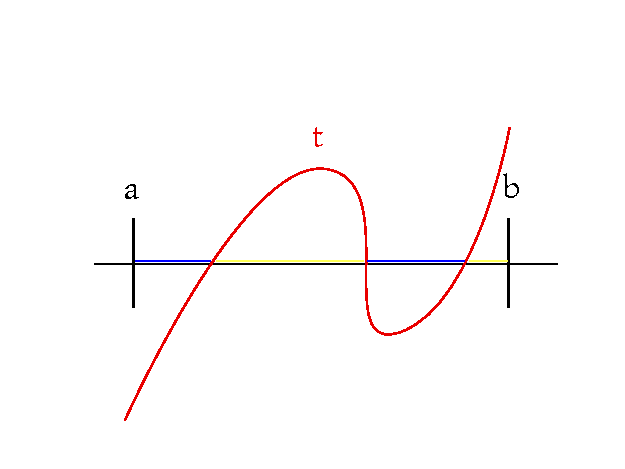
\includegraphics{img/signed_measure.pdf}
      \caption{Signed measure of $f$}
      \label{img:signed-measure}
    \end{center}
  \end{figure}

  \[ \nu(B) = \int_B f \, d\lambda = \int_{B \cap [f \geq 0]} f^+ \, d\lambda - \int_{B \cap [f < 0]} f^- \, d\lambda \]
\end{example}

\begin{theorem}[Hahn-Jordan]
  Let $\nu$ be signed.
  \[ X = P \cupdot N \qquad P,N \in \mathcal A \]
  \[ \nu^+(A) = \nu(A \cap P) \qquad \nu^-(A) = -\nu(A \cap N) \]
  Non-negative measures are $\nu^+ - \nu^- = \nu$.
\end{theorem}

\dateref{2018/12/10}

\begin{lemma}
  Let $A, B \in \mathcal A$, $B \subset A$ and $\Abs{\nu(A)} < \infty \implies \Abs{\nu(B)} < \infty$.
\end{lemma}

\begin{proof}
  \begin{center}
    \begin{tabular}{c|cc}
      $\nu(A)$  &$= \nu(B)$ &$+ \nu(A \setminus B)$ \\
    \hline
      $+\infty$ & $+\infty$ & $+ \infty$ \\
      $+\infty$ & $+\infty$ & $\in \mathbb R$ \\
      $-\infty$ & $-\infty$ & $-\infty$ \\
      $-\infty$ & $-\infty$ & $\in \mathbb R$
    \end{tabular}

    This shows a contradiction.
    $+\infty$ and $-\infty$ is not possible by definition of $\nu$.
  \end{center}
\end{proof}

\begin{lemma}
  \[ A_n \nearrow A \implies \nu(A_n) \to \nu(A) \]
\end{lemma}

\begin{lemma}
  \[ A_n \searrow A, \Abs{\nu(A_1)} < \infty \implies \nu(A_n) \to \nu(A) \]
\end{lemma}

\begin{proof}
  Immediate.
\end{proof}

\index{Positive signed measure}
\index{Negative signed measure}
\index{Zero-set signed measure}
\begin{definition}
  Let $\nu$ be a signed measure.
  \begin{itemize}
    \item $P \in \mathcal A$ is called positive if $\nu(A) \geq 0 \forall A \in \mathcal A, A \subset P$.
    \item $N \in \mathcal A$ is called negative if $\nu(A) \leq 0 \forall A \in \mathcal A, A \subset N$.
    \item $Z$ is a $\nu$-zero set if $\nu(A) = 0 \forall A \in \mathcal A$ with $A \subset Z$.
  \end{itemize}
\end{definition}

\begin{Remark}
  The subset of a positive set is positive.
\end{Remark}

\begin{lemma}
  \label{thm:exists-pos-set}
  Let $\nu: A \to [-\infty, \infty)$ be a signed measure.
  $A \in \mathcal A \implies \exists P \in \mathcal A, P \subset A$ positive, $\nu(P) \geq \nu(A)$.
\end{lemma}

\begin{proof}
  Case distinction of relation of $P$ and $A$.
  \begin{enumerate}
    \item $\nu(A) \leq 0: P = \emptyset$. Done.
    \item $\nu(A) = 0$
      \begin{claim}
        $\forall \varepsilon > 0 \exists A_{\varepsilon} \subset A$ with
        \begin{enumerate}
          \item $\nu(A_\varepsilon) \geq \nu(A)$
          \item $\nu(B) > -\varepsilon \forall B \subset A_{\varepsilon}$
        \end{enumerate}
      \end{claim}
      \begin{proof}
        Proof by contradiction.
        Assume $\exists \varepsilon > 0: \forall C \subset A$ with $\nu(C) \geq \nu(A): \exists B = B_C \subset C$ with $\nu(B) \leq -\varepsilon$. Inductive construction:
        \begin{enumerate}
          \item $C_0 = A \exists B_1 \subset A: \nu(B_1) \leq -\varepsilon$.
          \item $C_1 = A \setminus B_1: \nu(C_1) + \underbrace{\nu(B_1)}_{\leq -\varepsilon} = \nu(A)$
          \item $\nu(C_1) > \nu(C_0) = \nu(A): \exists B_2 \subset C_1: \nu(B_2) \leq -\varepsilon$. $C_2 = C_1 \setminus B_2$
          \item $\nu(C_2) + \underbrace{\nu(B_2)}_{\leq -\varepsilon} = \nu(C_1) \geq \nu(A)$. $\nu(C_2) > \nu(A)$.
          \item $B_1, B_2, \dots$ is pairwise disjoint. $\bigcupdot_{n} B_n \subset A$.
            \[ 0 < \nu(A) < \infty \implies \Abs{\nu\left(\bigcupdot_n B_n\right)} < \infty \]
            \[ \sum_n \underbrace{\nu(B_n)}_{\leq -\varepsilon} = -\infty \]
            This is a contradiction.
        \end{enumerate}
      \end{proof}

      Now let $\varepsilon = \frac1n$. $A_1$ for $\varepsilon = 1$ as above. $A_1 \subset A$ ($0 < \nu(A) < \infty$).
      $A_2 \subset A_1$ with respect to $A_1$ for $\varepsilon = \frac12$. $\nu(A_2) \geq \nu(A_1) \geq \nu(A)$.
      $A_3 \subset A_2$ with respect to $A_2$ for $\varepsilon = \frac13$. $\nu(B) > -\frac12 \forall B \subset A_2$.
      $A_3 \subset A_2$ with respect to $A_2$ for $\varepsilon = \frac13$.
      $A_n \subset A$, $A_{n+1} \subset A_n$. $\nu(B) > -\frac1{n+1} \forall B \in A_{n+1}$. $\nu(A_{n+1}) \geq \nu(A_n)$.

      $P \coloneqq \bigcap_n A_n$. So $\nu(A_n) \nearrow \nu(P)$. This implies that $\nu(P) \geq \nu(A)$.

      $P$ positive. $B \subset P \implies B \subset A_n$. $\nu(B) \geq -\frac1n \forall n$. Therefore $\geq 0$.

      Analogously for negative sets: If $\nu: \mathcal A \to (-\infty, \infty]$, then $\nu \leftrightarrow -\nu$ and $N \leftrightarrow P$.
  \end{enumerate}
\end{proof}

\begin{theorem}[Hahn decomposition theorem]
  Let $\nu$ be a signed measure. Then $X = P \cupdot N$ where $P$ is $\nu$-positive and $N$ is $\nu$-negative. $P, N \in \mathcal A$. Furthermore let $P, N$ be almost everywhere distinct. Hence $X = P' \cupdot N'$.
  \[ \nu(P' \triangle P) = \nu(N' \triangle N) = 0 \]
  where the symmetric unions are $\nu$-zero sets.
\end{theorem}

\begin{proof}
  Without loss of generality, $\nu: A \to [-\infty, +\infty)$.
  $\alpha = \sup\SetDef{\nu(A)}{A \in \mathcal A} \geq 0$. $\exists$ sequence $(A_n)$ in $\mathcal A$ such that $\nu(A_n) \nearrow \alpha$. By Theorem~\ref{thm:exists-pos-set}, $\exists P_n \subset A_n$ positive. $\alpha \geq \nu(P_n) \geq \nu(A_n)$. $\nu(P_n) \to \alpha$. $P = \bigcup_{n} P_n \supset P_n$.

  \[ \alpha \geq \nu(P) \geq \lim \nu(P_n) = \alpha \]
  Why does the second inequality hold? Because $P$ is positive (refer to the practicals, we might do this as an exercise).
  $P$ is disjoint countable union of positive sets.
  \[ P_1' = P_1, \qquad P_n' = P_n \setminus \bigcup_{k=2}^{n-1} P_k \]
  \[ \alpha = \nu(P) = \max\SetDef{\nu(A)}{A \in \mathcal A} < \infty \]
\end{proof}

\begin{claim}
  $N = P^C$ is negative.
\end{claim}
\begin{Remark}
  $\exists A \subset N: \nu(A) > 0$
\end{Remark}
\begin{proof}
  \[ \nu(A \cupdot P) = \nu(A) + \alpha > \alpha \]
  This is a contradiction.
\end{proof}

\[ \nu^+(A) \coloneqq \nu(A \cap P) \qquad \nu^-(A) \coloneqq -\nu(A \cap N) \]
is a non-negative measure.
\[ \nu = \nu^+ - \nu^- \]
one of them is finite.

\[ \Abs{\nu} \coloneqq \nu^+ + \nu^- \]
\[ \Abs{\nu}(A) = \nu^+(A) + \nu^-(A) \geq \Abs{\nu(A)} \]

\subsection{Total variation}

\index{Total variation}
\index{Singular measure}
\begin{definition}
  Let $\nu_1, \nu_2$ be signed measures are singular with respect to each other. $\nu_1 \bot \nu_2$, if they are concentrated on two disjoint sets:
  \[ \chi = A_1 \cupdot A_2, A_i \in \mathcal A: \nu_2(B) = \nu_C(B \cap A_i) \]
  So $A_2$ is a $\nu_1$-zero set and $A_2$ is a $\nu_2$ is a zero set.
\end{definition}

\begin{example}[$\nu^+ \bot \nu^-$ on $\mathbb R$]
  \[ \lambda \bot \text{ counting measure over } \mathbb Z \]
  \[ \mu(A) = \Abs{A \cap \mathbb Z} \]
\end{example}

\begin{theorem}[Jordan's decomposition theorem]
  Every signed measure $\nu$ has a unique decomposition $\nu = \nu^+ - \nu^-$ with $\nu^+ \geq 0, \nu^+ \bot \nu^-$.
\end{theorem}

\begin{Remark}[Minimality]
  If $\nu = \nu_1 - \nu_2$ with non-negative measures $\nu_i$ then $\nu^+ \leq \nu_1$, $\nu^- \leq \nu_2$.
  Is trivial to show.
\end{Remark}

\section{Theorem of Radon-Nikodym}

Related to Johann Radon: \url{https://en.wikipedia.org/wiki/Radon_transform}

Let $\mu$ be a positive measure on $(X, \mu)$. $\varphi: X \to \mathbb R$ measurable. $\int f \, d\mu$ exists.
\[ \nu(A) = \int_A f \, d\mu = \int f \cdot \mathbf{1}_A \, d\mu \]
Signed measure $\nu^+(A) = \int f^{\pm} \cdot \mathbf{1}_A \, d\mu$.

$\mu(A) = 0 \implies A \text{ is a } \nu\text{-zero set}$.

\index{Absolutely continuous signed measure}
\begin{Definition}
  $\nu$ (signed measure) is called \emph{absolutely continuous} with respect to $\mu$ ($\nu \ll \mu$)
  if $\mu(A) = 0 \implies A \text{ is a } \nu\text{-zero set} \forall A \in \mathcal A$.
\end{Definition}

\index{Radon-Nikodyn density}
\begin{theorem}
  Let $\mu$ be $\sigma$-finite measure. Let $\nu$ be a signed measure. $\nu \ll \mu$.
  \[ \implies \exists f: X \to \overline{\mathbb R} \text{ measurable } \]
  such that $\int_X f \, d\mu$ exists and $\nu(A) = \int_A f \, d\mu \forall A \in \mathcal A$.
  $f$ is $\mu$-almost everywhere distinct; i.e. if $\nu(A) = \int_A \tilde f d\mu  \forall A \in \mathcal A$
  then $\mu\left(\SetDef{x}{\tilde f(x) \neq f(x)}\right) = 0$.
  $f$ is called \emph{Radon-Nikodyn density} of $\nu$ with respect to $\mu$, $f = \frac{d\nu}{d\mu}$.

  Then $\int g \, d\nu = \int g f \, d\mu$ for \enquote{nice} $g: X \to \mathbb R$.
\end{theorem}

\dateref{2019/01/10}

\begin{theorem}[Hahn]
  Let $\nu$ be a signed measure.
  \[ X = P \cupdot N \]
  \[ P \in \mathbb A \text{ positive } [\nu(A) \geq 0 \forall A \subset P, A \in \mathcal A] \qquad N \in \mathbb A \text{ negative } \forall B \subseteq N, B \in \mathcal A \]
  $P, N$ are unique (up to zero sets)
  \[ \nu^+(A) = \nu(A \cap P) \qquad \nu^-(A) = -\nu(A \cap N) \]
  \[ \nu = \nu^+ - \nu^- (\text{Jordan decomposition}) \qquad \nu^+ \bot \nu^- \text{ on disjoint sets} \]
  and if $\nu = \nu_1 - \nu_2$ and $\nu_i$ are non-negative measures, then $\nu^+ \leq \nu_1$ and $\nu^- \leq \nu_2$.
\end{theorem}

\begin{remark}
  $\mu$ is a positive measure, $f: (X, \mathcal A) \to (\overline{\mathbb R}, {\mathcal B}_{\overline{\mathbb R}})$ such that $\int f \, d\mu$ exists. $\nu \coloneqq \mu_f$, $\mu_f(A) = \int_A f \, d\mu$ signed measure and $\mu(A) = 0 \implies A$ is a $\mu_f$-zero set.
\end{remark}

\begin{definition}
  $\nu \ll \mu$ ($\nu$ absolutely continuous w.r.t. $\mu$) if every $\mu$-zero set is alse a $\nu$-zero set.
\end{definition}

\begin{theorem}[Radon-Nikodyn]
  $\mu$ (positive measure!) $\sigma$-finite,
  $\nu \ll \mu$ (signed) $\implies \exists f: \nu = \mu_f$, $f$ is $\mu$ almost everywhere unique.
  \[ f \coloneqq \frac{d\nu}{d\mu} \]
\end{theorem}

\begin{proof}[Proof of Radon-Nikodyn theorem]
  Without loss of generality, $\nu \geq 0$. Why? Because $\nu^+ \ll \nu \ll \mu$. $\nu^+ = \mu_{f^+}$. $\nu^- = \nu_{f^-}$. $\nu = \mu_{f^+ - f^-}$.
  \begin{enumerate}
    \item $\mu, \nu$ is finite. $\mu(X), \nu(X) < \infty$. Let
      \[ \mathcal R = \SetDef{g}{X \to [0, \infty] \text{ measurable}, \int_A g \, d\mu \leq \nu(A) \forall A \in \mathcal A} \]
      $\mathcal R \neq \emptyset$ because $0 \in \mathcal R$.
      \[ \alpha \coloneqq \sup\left(\int g \, d\mu: g \in \mathcal R\right) \]
      \[ \exists g_n \in \mathcal R: \int g_n \, d\mu \to \alpha \]
      \[ f, g \in \mathbb R \xRightarrow{\text{claim}} \max\Set{f, g} \in \mathcal R \]
      \[ A_0 = [f \geq g] = \SetDef{x \in X}{f(x) \geq g(x)} \]
      \[ h(x) = \max\Set{f(x), g(x)} \qquad A_0^C = [f < g] \]
      \[ A_0^C = [f < g] \]

      \[ h = f \cdot \mathcal 1_{A_0} + g \cdot \mathcal 1_{A_0^C} \]
      Let $A \in \mathcal A$ be arbitrary.
      \begin{align*}
        \int_A h \, d\mu &= \int_A f \cdot \mathbf 1_{A_0} \, d\mu + \int_A g \cdot \mathbf 1_{A_0} c \, d\mu = \int_{A \cap A_0} f \, d\mu + \int_{A \cap A_0^C} g \, d\mu \\
          &\leq \nu(A \cap A_0) + \nu(A \cap A_0^C) = \nu(A)
      \end{align*}
      \[ f_n = \max{g_1, \dots, g_n} \in \mathcal R \qquad 0 \leq f_n \nearrow \]
      \[ \lim_{n \to \infty} \int f_n \, d\mu = \alpha \overset{\substack{\text{monotonic} \\ \text{convergence}}}= \int f \, d\mu \leq \nu(X) < \infty \qquad \text{and by } f \in \mathcal R \]
      Side condition: $\int_A f \, d\mu = \lim \int_A f_n \, d\mu \leq \nu(A)$. \\
      Now show: $\nu = \mu_f$. We know: $\nu \geq \mu_f$.

      Let $\tau = \nu - \mu_f$ is a non-negative measure, $\tau \ll \mu$.
      We want: $\tau \equiv 0$ suffices $\tau(X) = 0$. $\tau(X) = \nu(X) - \alpha$.
      $\varepsilon > 0$.
      \begin{align*}
        \sigma_\varepsilon &= \tau - \varepsilon \cdot \mu \qquad \text{signed measure} \\
          &= \underbrace{\sigma_\varepsilon^+}_{P_{\varepsilon}} - \underbrace{\sigma_\varepsilon^-}_{N_\varepsilon} \\
        P_\varepsilon \dotcup N_\varepsilon &= X
      \end{align*}

      Assumption:
      \[ \sigma_\varepsilon^+ \neq 0: \sigma_\varepsilon(P_\varepsilon) > 0 \implies \tau(P_\varepsilon) > 0 \implies \mu(P_\varepsilon) > 0 \]

      Let $f_\varepsilon = f + \varepsilon \mathbf 1_{P_\varepsilon}$.
      \begin{align*}
        \int_A f_{\varepsilon} \, d\mu &= \mu_f(A) + \varepsilon \mu(A \cap P_\varepsilon) < \mu_f(A) + \tau(A \cap P_\varepsilon) \\
      \intertext{$\tau(A \cap P_\varepsilon) - \varepsilon_\mu(A \cap P_\varepsilon) = \sigma_\varepsilon(A \cap P_{\varepsilon}) = \sigma^+_{\varepsilon} \geq 0$}
          &= \mu_f(A \cap N_\varepsilon) + \mu_\varepsilon(A \cap P_\varepsilon) + \nu(A \cap P_{\varepsilon}) - \mu_f(A\cap P_\varepsilon) \\
          &\leq \nu(A \cap N_{\varepsilon}) + \nu(A \cap P_\varepsilon) = \nu(A) \forall A \in \mathcal A
      \end{align*}
      So $f_{\varepsilon} \in \mathcal R$. So $\int f_\varepsilon \, d\mu \leq \alpha$ and $\underbrace{\int f \, d\mu}_{\alpha} + \underbrace{\varepsilon \mu(P_{\varepsilon})}_{> 0} > \alpha$ with $\int f_\varepsilon \, d\mu = \int f \, d\mu$.
      Contradiction!
      So $\sigma_\varepsilon^+ = 0$. $\sigma_\varepsilon = -\sigma_\varepsilon^-$.
      \[ (\tau - \varepsilon \mu)(X) \leq 0 \qquad T(X) \leq \varepsilon \cdot \mu(X) \forall \varepsilon > 0 \]
      Also $\tau(X) = 0$.
    \item Let $\mu$ be finite. Let $\nu \geq 0$ be arbitrary.
      Let $\beta = \sup\left\{\mu(B): B \in \mathcal A, \nu(B) < \infty\right\} \leq \mu(X) < \infty$.

      There exists some sequence $(B_n)$ of $A$ with $B_n \subset B_{n+1}$. $\nu(B_n) < \infty$. $\nu(B_n) \nearrow \beta$.
      Let $E = \bigcup_n B_n, F = E^C$.
      If $A \subset F, A \in \mathcal A$, we assume $\nu(A) < \infty \implies \nu(B_n \dotcup A) < \infty$
      \[ \implies \mu(B_n \cup A) \leq \beta \implies \mu(B_n) + \mu(A) \leq \beta \qquad n \to \infty \]
      \[ \mu(A) = 0 \implies \nu(A) = 0 \]
      Either $\mu(A) = \nu(A) = 0$ or $\mu(A) > 0, \nu(A) = \infty$.
      \[ E = \bigcupdot_n E_n \qquad E_1 = B_1 \qquad E_n = B_n \setminus B_{n-1} \qquad (n \geq 2) \]
      \[ \nu|_{E_n} \eqqcolon \nu_n \qquad \mu|_{E_n} \eqqcolon \mu_n \qquad \text{ are finite measures} \]
      \[ \nu_n(A) = \nu(E_n \cap A) \qquad \nu_n \ll \mu_n \]
      \[ \exists \tilde f_n: \nu_n(A) = \int_A \tilde f_n \, d\mu_n = \int_A \underbrace{\tilde f_n \cdot \mathbf 1_{E_n}}_{f_n} \, d\mu \forall A \in \mathcal A \]
      \[ f = \sum_{n = 1}^\infty f_n + \infty \cdot \mathbf 1_F \]
      \[ \nu(A) = \nu(A \cap E) + \nu(A \cap F) = \int_{A \cap E} f \, d\mu + \int_{A \cap F} \infty \, d\mu = \int_A f \, d\mu \forall A \in \mathcal A \]
    \item Let $\mu$ be $\sigma$-finite.
      \[ X = \bigcup_n^+ D_n \mu(D_n) < \infty \text{ then use } \mu|_{D_n}, \nu|_{D_n} \]
      The following remark is left as an exercise to the reader:
      $\mu_f = \mu_{f'} \implies f = f' \text{ is } \mu-\text{almost everywhere}$
  \end{enumerate}
\end{proof}

\dateref{2019/01/14}

\subsection{Convergence rates of sequences of functions}

\begin{definition}
  Let $(X, \mathcal A, \mu)$ is a measure space. $f_n, f: (X, \mathcal A) \to (\overline R, \mathcal B_{\overline R})$
  \begin{enumerate}
    \item $f_n \to f$ $\mu$-almost-everywhere if $\mu(\Set{x \in X}{f_n(x) \not\to f(x)}) = 0$.
      \[ \mu[f_n \not\to f] \]
    \item $f_n \to f$ in the measure if $\lim_{n \to \infty}\left(\SetDef{x}{\Abs{f_n(x) - f(x)} \geq a}\right) = 0$
      \[ \mu[\Abs{f_n - f} \geq a] \forall a > 0 \]
  \end{enumerate}
\end{definition}

TODO: there was another board with notes

\begin{lemma}
  In both cases, $f$ $\mu$-almost-everywhere unambiguous. So, if $f_n \to f$ and $f_n \to g$ $\mu$-almost-everywhere in the measure.
  \[ \implies f = g \mu\text{-almost-everywhere}: \mu[f \neq g] = 0 \]
\end{lemma}

\[ \Abs{f - g} \leq \Abs{f - f_n} + \Abs{f_n - g} \]
\[ \left[\Abs{f - g} \geq a\right] \subset \left[\Abs{f_n - f} \geq \frac a2\right] \cup \left[\Abs{f_n - g} \geq \frac a2\right] \]
\[ \mu\left[\Abs{f - g} \geq a\right] \leq \mu\left[\Abs{f_n - f} \geq \frac a2\right] + \mu\left[\Abs{f_n - g} \geq \frac a2\right] \]
Also $\mu[\Abs{f - g} \geq a] = 0 \forall a = \frac 1r > 0$ with $r \in \mathbb N$.
\[ \implies \mu[\Abs{f - g} > 0] = 0 \]

\begin{theorem}
  If $\mu(X) < \infty$, then $f_n - f$ $\mu$-almost-everywhere $\iff g_k = \sup_{n \geq k} \Abs{f_n - f} \to 0$ in the measure.
\end{theorem}

\begin{proof}
  \[ A = [f_n - f] = \left[\forall r \exists k \forall n \geq k: \Abs{f_n - f} \leq \frac 1r\right] \]
  \[ = \bigcap_r A_r, A_r = \left[\exists k \forall n \geq k: \Abs{f_n - f} \leq \frac 1r\right] \supset A_{r+1} \]
  \[ A = \bigcap_r A_r \qquad A^C = \bigcap_r A_r^C \]
  \[ f_n \to f \mu\text{-almost-everywhere} \iff \mu(A^C) = 0 \iff \forall r: \mu(A_r^C) = 0 \]
  \[ A_r^C = \bigcap_k \left[\exists n \geq k: \Abs{f_n - f} > \frac 1r\right] = \bigcap_k \underbrace{\left[g_k > \frac 1r\right]}_{B_{k,r} \supset B_{k+1,r}} \]
  with $g_k > g_{k+1}$,
  \[ \iff \forall r: \mu\left(\bigcap_k B_{k,r}\right) = 0 \qquad B_{k,r} \searrow A^C \]
  \[ \iff \forall r: \mu(B_{k,r}) \xrightarrow{k\to\infty} 0 \]
  where $\implies$ is given because $\mu(X) < \infty$.
  \[ \forall r: \mu\left[g_k < \frac 1r\right] \xrightarrow{k \to \infty} 0 \]
  $g_k \to 0$ in the measure.
\end{proof}

\begin{definition}
  Let $(f_n)$ be a Cauchy sequence in the measure if
  \[ \lim_{m,n \to \infty} \mu\left[\Abs{f_n - f_m} > a\right] = 0 \forall a > 0, a = \frac 1r, r \in \mathbb N \]
  \[ \lim_{n \to \infty} \sup_{m > n} \mu\left[\left(f_n - f_m\right) > a\right] = 0 \forall a > 0 \]
\end{definition}

\begin{theorem}
  \begin{enumerate}
    \item $\exists f: f_n \to f$ in the measure $\iff (f_n)$ in Cauchy sequence in the measure
    \item $f_n \to f$ in the measure $\implies f_{n_k} \to f$ $\mu$-almost-everywhere for some subsequence.
  \end{enumerate}
\end{theorem}

\begin{example}
  Let $X = (0,1], \mathbb B_{(0, 1]}, \mu = \lambda$ is a Lebesgue measure.
  \[ I_1 = (0, 1] \qquad I_2 = (0, \frac12] \qquad I_3 = (\frac12, 1] \qquad I_4 = (0, \frac14] \qquad \dots \]
  \[ I_7 = (\frac34, 1] \qquad I_8 = (0, \frac18] \qquad I_9 = (\frac18, \frac28] \qquad I_{16} = (0, \frac1{16}] \]
  TODO
  \[ f_{2^k} = \mathbf 1_{(0, \frac{1}{2^k}]} \]
  $x \in (0, 1]$: if $\frac{1}{2^k} < x$, then $f_{2^k}(x) = 0$.
  $f_{2^k} \to 0$ $(\lambda-f)$ everywhere.
\end{example}

\begin{proof}
  \begin{description}
    \item[1. $\implies$]
      $f_n \to f$ in the measure. $\forall a > 0$
      \[ \mu\left(\Abs{f_n - f_m} \geq a\right) \leq \mu\left(\Abs{f_n - f} \geq \frac a2\right) + \mu\left(\Abs{f_n - f} \geq \frac a2\right) \xrightarrow{n,m \to \infty} 0 \]
    \item[1. $\impliedby$, and 2.]
      \[ a_k > \varepsilon_k = \frac1{2^k}: \exists n_k \forall n, m \geq n_k \]
      \[ \mu\left[\Abs{f_n - f_m} \geq \frac{1}{2^k}\right] < \frac{1}{2^k} \]
      wlog. $n_{k+1} > n_k \implies$
      \[ \sum_{k=1}^\infty \mu\left[\Abs{f_{n_{k+1}} - f_{n_k}} \geq \frac{1}{2^k}\right] < \sum_k \frac{1}{2^k} < \infty \]
  \end{description}
\end{proof}

\paragraph{Excursion}

\begin{lemma}[Borel-Cantelli Lemma]
  \[ \sum_{k=1}^\infty \mu(A_k) < \infty \implies \mu\left(\lim\sup{A_k} = 0\right) \]
  \[ \mu\left(\bigcap_{n=1}^{\infty} \underbrace{\bigcup_{k=m}^{\infty} A_k}_{B_m \supset B_{m+1}} \right) = 0 \]
  \[ \mu(B_1) \leq \sum_{k} \mu(A_k) < \infty \qquad B_m \searrow \lim\sup A_k \]
  So, $\mu(\lim\sup{A_k}) > \lim_m \mu(B_m)$
  \[ \mu(B_m) \leq \sum_{k=m}^{\infty} \mu(A_k) \xrightarrow{m \to \infty} 0 \]
\end{lemma}

\[ \implies \mu\underbrace{\left(\lim\sup\underbrace{[\Abs{f_{n_{k+1}} - f_{n_k}} \geq \frac{1}{2^k}]}_{D_k^C}\right)}_{D^C} = 0 \]
\[ D = \lim\inf D_k = \bigcup_{m=1}^\infty \bigcap_{k=m}^\infty D_k \]
\[ x \in D \implies \exists m: x \in D_k \forall k \geq m \]

\[ \Abs{f_n(x) - f_{n_k}(x)} < \frac{1}{2^k} \forall k \geq m \]
\[ \sum_{k = 1}^{\infty} \Abs{f_{n_{k+1}}(x) - f_{n_k}(x)} < \infty \]
\[ \sum_{k = 1}^{\infty} \left(f_{n_{k+1}}(x) - f_{n_k}(x)\right) \text{ converges as well} \]
\[ \sum_{k = 1}^{k - 1} \left(\dots\right) = f_{n_k}(x) - f_{n_1}(1) \text{ converges, } k \to \infty \]
so,
\[ \exists \lim_{k \to \infty} f_{n_k}(x) = f(x), \mu(D^C) = 0, f|_{D^C} = 0 \]
\[ f_{n_k} \to f \mu\text{-almost-everywhere} \]
It remains to show that $f_n \to f$ in the measure.

\[ \mu\left[\Abs{f_n - f} \geq a\right] = \mu\left[\lim_{k \to \infty} \inf \Abs{f_n - f_{n_k}} \geq a\right] \]
\[ \overset{\text{Fatou}}{\leq} \lim_{k \to \infty} \inf \underbrace{\mu \left[\Abs{f_n - f_{n_k}} \geq a\right]}_{< \varepsilon, \text{ if } n, n_k \text{ sufficiently large}} \]

In the next lecture, we will discuss:

$L^p$ convergence:

\begin{definition}
  \[ \Norm{f}_p \coloneqq \int_X \left(\Abs{f(x)}^p\right)^{\frac1p} \qquad 1 \leq 1 < \infty \]
  \begin{align*}
    \Norm{f}_\infty &\coloneqq \operatorname{ess\,sup}\Abs{f} = \inf\SetDef{c > 0}{\Abs{f} \leq c \quad \mu-\text{almost-everwhere}} \\
      &= \inf\SetDef{\sup_A\Abs{f(x)}}{A \in \mathcal A: \mu(A^C) = 0}
  \end{align*}
  \[ f \sim g \iff \mu[f \neq g] = 0, \text{ so } f = g \, \mu\text{-almost-everywhere} \]
\end{definition}


\printindex
\end{document}
